\section{Results}
\label{sec:results}

We organize the presentation of our findings by topic, starting with Tor
Browser, and then onion service-specific topics such as service discovery and
the operation of onion services.  We interweave the results from our online
survey and from our interviews, focusing primarily on our survey data but
bringing up anecdotes and findings from our interviews as appropriate.

\subsection{The Tor Project}

Our work focuses on the usability of onion services, but our interviews and parts
of our survey data also provided some insight into how our respondents perceive The Tor
Project and its work.  We summarize these findings here.

\subsubsection{Documentation and localization}

The Tor Project's documentation covers an array of topics including
installation, the use on Android, the operation of Tor relays, several
\textsc{faq}s, and a wiki.  Having worked with this documentation, some of our
interview and survey participants lamented its scope:

\begin{displayquote}[P14]
Tor does a good job on their web site of telling you to modify your
[configuration] file, and then getting the onion set up.  But it's just very
basic.  I have to go [to] other people's blog post to find out.
\end{displayquote}

Another participant struggled with the lack of localization.  While Tor
Browser's user interface is available in Spanish, the documentation is not:

\begin{displayquote}[P11]
Think more [about] the Spanish community\dots because in my case I'm trying to
train people to use Tor but I work in the indigenous communities and there are
some things that [are] hard for me to explain in terms of how you use Tor\dots
\end{displayquote}

\subsubsection{Public perception}

The Tor Project goes to great lengths to minimize the trust its users have to
place in it by publishing design documents and source code and coordinating
development in public.  Laypeople however lack the skill while experts typically
lack the time to audit source code, which is why trust and reputation matter.
The Tor Project enjoyed a lot of trust among our interview participants, which,
admittedly, comes as no surprise because we recruited our interviewees from
Tor-friendly social media and an Internet freedom event.

\begin{displayquote}[P08]
Because, you guys\dots have the sort of\dots not a monopoly on trust, but you
have like a really great brand name when it comes to this stuff\dots
\end{displayquote}

While the work of Tor developers is often held in high esteem, the content that
is hosted on onion services is perceived very differently.  Upon being told what
an onion service is, one participant sought clarification:

\begin{displayquote}[P03]
So it's like the Hidden Wiki and stuff like that, where you can buy drugs
and\dots or supposedly.
\end{displayquote}

\hyperref[q6_3]{Questions 6.3} and \hyperref[q6_5]{6.5} asked how safe our
respondents feel when using Tor Browser and onion services, respectively.
\Cref{fig:perceived-security} shows the results.  The use of Tor Browser makes
86\% of our respondents feel at least somewhat safe.  The same is true for 67\%
when using onion services---clearly not as many as for Tor Browser.

\begin{figure}[t]
    \centering
    % Created by tikzDevice version 0.10.1 on 2018-01-12 16:35:49
% !TEX encoding = UTF-8 Unicode
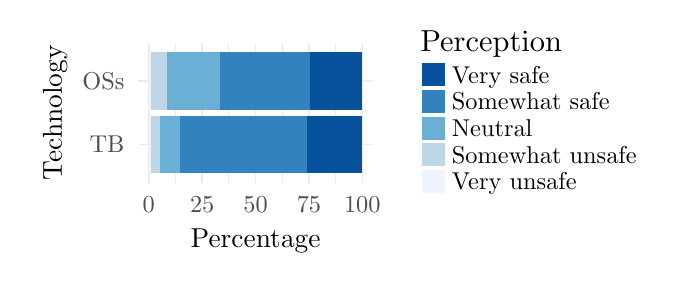
\begin{tikzpicture}[x=1pt,y=1pt]
\definecolor{fillColor}{RGB}{255,255,255}
\path[use as bounding box,fill=fillColor,fill opacity=0.00] (0,0) rectangle (231.26, 86.72);
\begin{scope}
\path[clip] ( 39.91, 30.77) rectangle (124.79, 81.22);
\definecolor{drawColor}{gray}{0.92}

\path[draw=drawColor,line width= 0.3pt,line join=round] ( 53.42, 30.77) --
	( 53.42, 81.22);

\path[draw=drawColor,line width= 0.3pt,line join=round] ( 72.71, 30.77) --
	( 72.71, 81.22);

\path[draw=drawColor,line width= 0.3pt,line join=round] ( 92.00, 30.77) --
	( 92.00, 81.22);

\path[draw=drawColor,line width= 0.3pt,line join=round] (111.29, 30.77) --
	(111.29, 81.22);

\path[draw=drawColor,line width= 0.6pt,line join=round] ( 39.91, 44.53) --
	(124.79, 44.53);

\path[draw=drawColor,line width= 0.6pt,line join=round] ( 39.91, 67.46) --
	(124.79, 67.46);

\path[draw=drawColor,line width= 0.6pt,line join=round] ( 43.77, 30.77) --
	( 43.77, 81.22);

\path[draw=drawColor,line width= 0.6pt,line join=round] ( 63.06, 30.77) --
	( 63.06, 81.22);

\path[draw=drawColor,line width= 0.6pt,line join=round] ( 82.35, 30.77) --
	( 82.35, 81.22);

\path[draw=drawColor,line width= 0.6pt,line join=round] (101.64, 30.77) --
	(101.64, 81.22);

\path[draw=drawColor,line width= 0.6pt,line join=round] (120.93, 30.77) --
	(120.93, 81.22);
\definecolor{fillColor}{RGB}{239,243,255}

\path[fill=fillColor] ( 43.77, 34.21) rectangle ( 44.51, 54.85);
\definecolor{fillColor}{RGB}{189,215,231}

\path[fill=fillColor] ( 44.51, 34.21) rectangle ( 47.92, 54.85);
\definecolor{fillColor}{RGB}{107,174,214}

\path[fill=fillColor] ( 47.92, 34.21) rectangle ( 54.90, 54.85);
\definecolor{fillColor}{RGB}{49,130,189}

\path[fill=fillColor] ( 54.90, 34.21) rectangle (100.90, 54.85);
\definecolor{fillColor}{RGB}{8,81,156}

\path[fill=fillColor] (100.90, 34.21) rectangle (120.93, 54.85);
\definecolor{fillColor}{RGB}{239,243,255}

\path[fill=fillColor] ( 43.77, 57.15) rectangle ( 44.67, 77.78);
\definecolor{fillColor}{RGB}{189,215,231}

\path[fill=fillColor] ( 44.67, 57.15) rectangle ( 50.19, 77.78);
\definecolor{fillColor}{RGB}{107,174,214}

\path[fill=fillColor] ( 50.19, 57.15) rectangle ( 69.60, 77.78);
\definecolor{fillColor}{RGB}{49,130,189}

\path[fill=fillColor] ( 69.60, 57.15) rectangle (101.98, 77.78);
\definecolor{fillColor}{RGB}{8,81,156}

\path[fill=fillColor] (101.98, 57.15) rectangle (120.93, 77.78);
\end{scope}
\begin{scope}
\path[clip] (  0.00,  0.00) rectangle (231.26, 86.72);
\definecolor{drawColor}{gray}{0.30}

\node[text=drawColor,anchor=base east,inner sep=0pt, outer sep=0pt, scale=  0.88] at ( 34.96, 41.50) {TB};

\node[text=drawColor,anchor=base east,inner sep=0pt, outer sep=0pt, scale=  0.88] at ( 34.96, 64.43) {OSs};
\end{scope}
\begin{scope}
\path[clip] (  0.00,  0.00) rectangle (231.26, 86.72);
\definecolor{drawColor}{gray}{0.30}

\node[text=drawColor,anchor=base,inner sep=0pt, outer sep=0pt, scale=  0.88] at ( 43.77, 19.76) {0};

\node[text=drawColor,anchor=base,inner sep=0pt, outer sep=0pt, scale=  0.88] at ( 63.06, 19.76) {25};

\node[text=drawColor,anchor=base,inner sep=0pt, outer sep=0pt, scale=  0.88] at ( 82.35, 19.76) {50};

\node[text=drawColor,anchor=base,inner sep=0pt, outer sep=0pt, scale=  0.88] at (101.64, 19.76) {75};

\node[text=drawColor,anchor=base,inner sep=0pt, outer sep=0pt, scale=  0.88] at (120.93, 19.76) {100};
\end{scope}
\begin{scope}
\path[clip] (  0.00,  0.00) rectangle (231.26, 86.72);
\definecolor{drawColor}{RGB}{0,0,0}

\node[text=drawColor,anchor=base,inner sep=0pt, outer sep=0pt, scale=  0.99] at ( 82.35,  7.44) {Percentage};
\end{scope}
\begin{scope}
\path[clip] (  0.00,  0.00) rectangle (231.26, 86.72);
\definecolor{drawColor}{RGB}{0,0,0}

\node[text=drawColor,rotate= 90.00,anchor=base,inner sep=0pt, outer sep=0pt, scale=  0.99] at ( 12.32, 56.00) {Technology};
\end{scope}
\begin{scope}
\path[clip] (  0.00,  0.00) rectangle (231.26, 86.72);
\definecolor{drawColor}{RGB}{0,0,0}

\node[text=drawColor,anchor=base west,inner sep=0pt, outer sep=0pt, scale=  1.10] at (141.86, 78.11) {Perception};
\end{scope}
\begin{scope}
\path[clip] (  0.00,  0.00) rectangle (231.26, 86.72);
\definecolor{fillColor}{RGB}{8,81,156}

\path[fill=fillColor] (142.58, 65.57) rectangle (150.79, 73.78);
\end{scope}
\begin{scope}
\path[clip] (  0.00,  0.00) rectangle (231.26, 86.72);
\definecolor{fillColor}{RGB}{49,130,189}

\path[fill=fillColor] (142.58, 55.93) rectangle (150.79, 64.15);
\end{scope}
\begin{scope}
\path[clip] (  0.00,  0.00) rectangle (231.26, 86.72);
\definecolor{fillColor}{RGB}{107,174,214}

\path[fill=fillColor] (142.58, 46.30) rectangle (150.79, 54.51);
\end{scope}
\begin{scope}
\path[clip] (  0.00,  0.00) rectangle (231.26, 86.72);
\definecolor{fillColor}{RGB}{189,215,231}

\path[fill=fillColor] (142.58, 36.66) rectangle (150.79, 44.87);
\end{scope}
\begin{scope}
\path[clip] (  0.00,  0.00) rectangle (231.26, 86.72);
\definecolor{fillColor}{RGB}{239,243,255}

\path[fill=fillColor] (142.58, 27.03) rectangle (150.79, 35.24);
\end{scope}
\begin{scope}
\path[clip] (  0.00,  0.00) rectangle (231.26, 86.72);
\definecolor{drawColor}{RGB}{0,0,0}

\node[text=drawColor,anchor=base west,inner sep=0pt, outer sep=0pt, scale=  0.88] at (153.31, 66.65) {Very safe};
\end{scope}
\begin{scope}
\path[clip] (  0.00,  0.00) rectangle (231.26, 86.72);
\definecolor{drawColor}{RGB}{0,0,0}

\node[text=drawColor,anchor=base west,inner sep=0pt, outer sep=0pt, scale=  0.88] at (153.31, 57.01) {Somewhat safe};
\end{scope}
\begin{scope}
\path[clip] (  0.00,  0.00) rectangle (231.26, 86.72);
\definecolor{drawColor}{RGB}{0,0,0}

\node[text=drawColor,anchor=base west,inner sep=0pt, outer sep=0pt, scale=  0.88] at (153.31, 47.37) {Neutral};
\end{scope}
\begin{scope}
\path[clip] (  0.00,  0.00) rectangle (231.26, 86.72);
\definecolor{drawColor}{RGB}{0,0,0}

\node[text=drawColor,anchor=base west,inner sep=0pt, outer sep=0pt, scale=  0.88] at (153.31, 37.74) {Somewhat unsafe};
\end{scope}
\begin{scope}
\path[clip] (  0.00,  0.00) rectangle (231.26, 86.72);
\definecolor{drawColor}{RGB}{0,0,0}

\node[text=drawColor,anchor=base west,inner sep=0pt, outer sep=0pt, scale=  0.88] at (153.31, 28.10) {Very unsafe};
\end{scope}
\end{tikzpicture}

    \caption{The level of safety our respondents perceive when using Tor
    Browser (\textsc{tb}) and onion services (\textsc{os}s).}
    \label{fig:perceived-security}
\end{figure}

Asked about why our respondents feel that way about Tor Browser, our results
reveal that non-experts lack the ability to evaluate (or even understand) Tor's
design which is why they defer to expert opinion, their gut feeling, or the
trust they place in Tor developers.  The Tor Project is perceived to take
security and privacy more seriously than any other browser vendor, which is
appreciated among our respondents.  Most of our respondents' criticism focused
not on Tor Browser but on the underlying Firefox code base.  Many participants
were unhappy with Firefox's exploit mitigation techniques, the lack of
sandboxing, and the complex code base.  Chrome was sometimes brought up as the
gold standard for browser security.\footnote{Note that we conducted our survey
before Mozilla released Firefox Quantum on November 14, 2017, which brought
substantial improvements in both security and usability.}  Malicious exit relays
were a concern for a handful of participants while another couple of
participants were concerned that their use of Tor makes them stick out and turns 
them into targets for government agencies.  Tor Browser comes with modules that
disguise the fact that one is using Tor, but a standard Tor connection does not
use these modules, making it easy to identify for Internet service
providers~\cite{pluggable}.  One interview participant worried:

\begin{displayquote}[P03]
I guess you could put yourself on some kind of watch lists, that you are a
person of interest, just because you're using [Tor].
\end{displayquote}

Some survey respondents were not sure if their Tor setup works properly---a
common theme that we also noticed in our interviews: Non-technical users desire
visual feedback confirming that their network traffic comes out ``somewhere
else,'' a point that we will elaborate on in \Cref{sec:under-the-hood}.

With respect to onion services, the majority expressed that the added security
and anonymity makes them feel safe.  Another factor contributing to the
perceived security is that onion services make use of far fewer advertising
companies.  Orthogonal to the technology, many participants voiced concern about
illegal and questionable content on onion services, described by some as a
``Wild West.''  Phishing sites, honeypots, and compromised onion sites further
contribute to this perception.

\subsection{Tor Browser usage}

Our survey started with two questions about how often our respondents use Tor
Browser.  The results are illustrated in \Cref{fig:tor-usage}.  Almost half of
our participants use Tor Browser either daily or even as their main browser.
Both Gallagher \ea~\cite[\S~4.3.2]{Gallagher2017a} and our interview data
suggests that non-experts frequently use Tor for specific tasks but do not embed
it in their daily workflow:

\begin{displayquote}[P07]
Right now, I use it very little, just because I don't have a lot of reasons to,
because of the fact that I have other security practices that do the trick for
the kind of work that I do.
\end{displayquote}

\begin{figure}[t]
    \centering
    % Created by tikzDevice version 0.10.1 on 2018-01-12 15:55:47
% !TEX encoding = UTF-8 Unicode
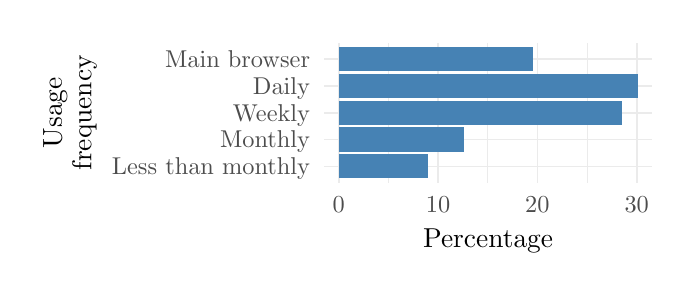
\begin{tikzpicture}[x=1pt,y=1pt]
\definecolor{fillColor}{RGB}{255,255,255}
\path[use as bounding box,fill=fillColor,fill opacity=0.00] (0,0) rectangle (231.26, 86.72);
\begin{scope}
\path[clip] (106.99, 30.77) rectangle (225.76, 81.22);
\definecolor{drawColor}{gray}{0.92}

\path[draw=drawColor,line width= 0.3pt,line join=round] (130.33, 30.77) --
	(130.33, 81.22);

\path[draw=drawColor,line width= 0.3pt,line join=round] (166.23, 30.77) --
	(166.23, 81.22);

\path[draw=drawColor,line width= 0.3pt,line join=round] (202.13, 30.77) --
	(202.13, 81.22);

\path[draw=drawColor,line width= 0.6pt,line join=round] (106.99, 36.59) --
	(225.76, 36.59);

\path[draw=drawColor,line width= 0.6pt,line join=round] (106.99, 46.30) --
	(225.76, 46.30);

\path[draw=drawColor,line width= 0.6pt,line join=round] (106.99, 56.00) --
	(225.76, 56.00);

\path[draw=drawColor,line width= 0.6pt,line join=round] (106.99, 65.70) --
	(225.76, 65.70);

\path[draw=drawColor,line width= 0.6pt,line join=round] (106.99, 75.40) --
	(225.76, 75.40);

\path[draw=drawColor,line width= 0.6pt,line join=round] (112.38, 30.77) --
	(112.38, 81.22);

\path[draw=drawColor,line width= 0.6pt,line join=round] (148.28, 30.77) --
	(148.28, 81.22);

\path[draw=drawColor,line width= 0.6pt,line join=round] (184.18, 30.77) --
	(184.18, 81.22);

\path[draw=drawColor,line width= 0.6pt,line join=round] (220.08, 30.77) --
	(220.08, 81.22);
\definecolor{fillColor}{RGB}{70,130,180}

\path[fill=fillColor] (112.38, 32.23) rectangle (144.69, 40.96);

\path[fill=fillColor] (112.38, 41.93) rectangle (157.76, 50.66);

\path[fill=fillColor] (112.38, 51.63) rectangle (214.84, 60.36);

\path[fill=fillColor] (112.38, 61.33) rectangle (220.36, 70.07);

\path[fill=fillColor] (112.38, 71.04) rectangle (182.53, 79.77);
\end{scope}
\begin{scope}
\path[clip] (  0.00,  0.00) rectangle (231.26, 86.72);
\definecolor{drawColor}{gray}{0.30}

\node[text=drawColor,anchor=base east,inner sep=0pt, outer sep=0pt, scale=  0.88] at (102.04, 33.56) {Less than monthly};

\node[text=drawColor,anchor=base east,inner sep=0pt, outer sep=0pt, scale=  0.88] at (102.04, 43.27) {Monthly};

\node[text=drawColor,anchor=base east,inner sep=0pt, outer sep=0pt, scale=  0.88] at (102.04, 52.97) {Weekly};

\node[text=drawColor,anchor=base east,inner sep=0pt, outer sep=0pt, scale=  0.88] at (102.04, 62.67) {Daily};

\node[text=drawColor,anchor=base east,inner sep=0pt, outer sep=0pt, scale=  0.88] at (102.04, 72.37) {Main browser};
\end{scope}
\begin{scope}
\path[clip] (  0.00,  0.00) rectangle (231.26, 86.72);
\definecolor{drawColor}{gray}{0.30}

\node[text=drawColor,anchor=base,inner sep=0pt, outer sep=0pt, scale=  0.88] at (112.38, 19.76) {0};

\node[text=drawColor,anchor=base,inner sep=0pt, outer sep=0pt, scale=  0.88] at (148.28, 19.76) {10};

\node[text=drawColor,anchor=base,inner sep=0pt, outer sep=0pt, scale=  0.88] at (184.18, 19.76) {20};

\node[text=drawColor,anchor=base,inner sep=0pt, outer sep=0pt, scale=  0.88] at (220.08, 19.76) {30};
\end{scope}
\begin{scope}
\path[clip] (  0.00,  0.00) rectangle (231.26, 86.72);
\definecolor{drawColor}{RGB}{0,0,0}

\node[text=drawColor,anchor=base,inner sep=0pt, outer sep=0pt, scale=  0.99] at (166.37,  7.44) {Percentage};
\end{scope}
\begin{scope}
\path[clip] (  0.00,  0.00) rectangle (231.26, 86.72);
\definecolor{drawColor}{RGB}{0,0,0}

\node[text=drawColor,rotate= 90.00,anchor=base,inner sep=0pt, outer sep=0pt, scale=  0.99] at ( 12.32, 56.00) {Usage};

\node[text=drawColor,rotate= 90.00,anchor=base,inner sep=0pt, outer sep=0pt, scale=  0.99] at ( 23.01, 56.00) {frequency};
\end{scope}
\end{tikzpicture}

    \caption{The usage frequency of Tor Browser among our respondents, almost
    half of whom use Tor Browser either daily or as their main browser.}
    \label{fig:tor-usage}
\end{figure}

\Cref{fig:tor-threats} illustrates what entities our respondents seek to protect
themselves from when using Tor Browser.  The majority want to protect themselves
from ad companies, governments, and most prominently, their \textsc{isp}s.
More tangible entities such as family, employers, and schools are less prevalent.
People who selected ``Other'' gave a variety of responses.  A number of respondents
specifically pointed out Google and Facebook.  \textsc{isp}s, backbone
\textsc{isp}s, and web sites were another common theme.  A number of respondents
are struggling with personal threats that include identity theft, targeted
harassment, and stalking.  Research is another common theme: Several respondents
want to learn about a topic without revealing their interest in it.  Some
respondents use Tor for search engine optimization, computer security research,
and to research medical conditions.  Finally, Tor has use cases that do not
involve a threat actor.  Some respondents want IPv6 connectivity, evasion of
geographical content restrictions, and access to onion services.  One respondent
stated that they do not need anonymity themselves but use Tor to provide cover
traffic for ``people who need protection.''


\begin{figure}[t]
    \centering
    % Created by tikzDevice version 0.10.1 on 2018-02-09 14:33:04
% !TEX encoding = UTF-8 Unicode
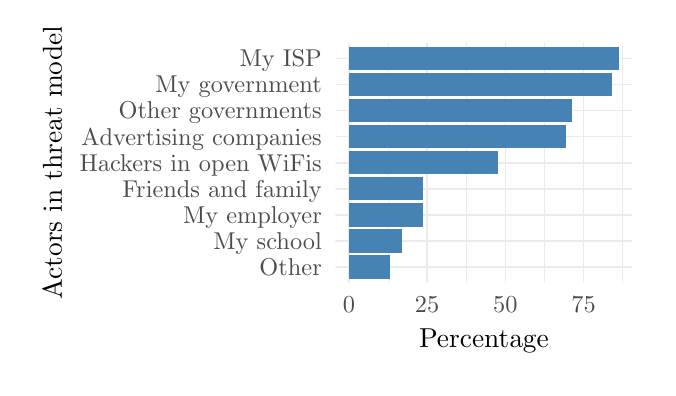
\begin{tikzpicture}[x=1pt,y=1pt]
\definecolor{fillColor}{RGB}{255,255,255}
\path[use as bounding box,fill=fillColor,fill opacity=0.00] (0,0) rectangle (224.04,122.86);
\begin{scope}
\path[clip] (111.23, 30.77) rectangle (218.54,117.36);
\definecolor{drawColor}{gray}{0.92}

\path[draw=drawColor,line width= 0.3pt,line join=round] (130.23, 30.77) --
	(130.23,117.36);

\path[draw=drawColor,line width= 0.3pt,line join=round] (158.48, 30.77) --
	(158.48,117.36);

\path[draw=drawColor,line width= 0.3pt,line join=round] (186.72, 30.77) --
	(186.72,117.36);

\path[draw=drawColor,line width= 0.3pt,line join=round] (214.97, 30.77) --
	(214.97,117.36);

\path[draw=drawColor,line width= 0.6pt,line join=round] (111.23, 36.42) --
	(218.54, 36.42);

\path[draw=drawColor,line width= 0.6pt,line join=round] (111.23, 45.83) --
	(218.54, 45.83);

\path[draw=drawColor,line width= 0.6pt,line join=round] (111.23, 55.24) --
	(218.54, 55.24);

\path[draw=drawColor,line width= 0.6pt,line join=round] (111.23, 64.65) --
	(218.54, 64.65);

\path[draw=drawColor,line width= 0.6pt,line join=round] (111.23, 74.07) --
	(218.54, 74.07);

\path[draw=drawColor,line width= 0.6pt,line join=round] (111.23, 83.48) --
	(218.54, 83.48);

\path[draw=drawColor,line width= 0.6pt,line join=round] (111.23, 92.89) --
	(218.54, 92.89);

\path[draw=drawColor,line width= 0.6pt,line join=round] (111.23,102.30) --
	(218.54,102.30);

\path[draw=drawColor,line width= 0.6pt,line join=round] (111.23,111.71) --
	(218.54,111.71);

\path[draw=drawColor,line width= 0.6pt,line join=round] (116.11, 30.77) --
	(116.11,117.36);

\path[draw=drawColor,line width= 0.6pt,line join=round] (144.35, 30.77) --
	(144.35,117.36);

\path[draw=drawColor,line width= 0.6pt,line join=round] (172.60, 30.77) --
	(172.60,117.36);

\path[draw=drawColor,line width= 0.6pt,line join=round] (200.85, 30.77) --
	(200.85,117.36);
\definecolor{fillColor}{RGB}{70,130,180}

\path[fill=fillColor] (116.11, 32.18) rectangle (130.90, 40.66);

\path[fill=fillColor] (116.11, 41.60) rectangle (135.19, 50.07);

\path[fill=fillColor] (116.11, 51.01) rectangle (142.69, 59.48);

\path[fill=fillColor] (116.11, 60.42) rectangle (142.91, 68.89);

\path[fill=fillColor] (116.11, 69.83) rectangle (169.92, 78.30);

\path[fill=fillColor] (116.11, 79.24) rectangle (194.36, 87.71);

\path[fill=fillColor] (116.11, 88.65) rectangle (196.72, 97.12);

\path[fill=fillColor] (116.11, 98.07) rectangle (211.30,106.54);

\path[fill=fillColor] (116.11,107.48) rectangle (213.66,115.95);
\end{scope}
\begin{scope}
\path[clip] (  0.00,  0.00) rectangle (224.04,122.86);
\definecolor{drawColor}{gray}{0.30}

\node[text=drawColor,anchor=base east,inner sep=0pt, outer sep=0pt, scale=  0.88] at (106.28, 33.39) {Other};

\node[text=drawColor,anchor=base east,inner sep=0pt, outer sep=0pt, scale=  0.88] at (106.28, 42.80) {My school};

\node[text=drawColor,anchor=base east,inner sep=0pt, outer sep=0pt, scale=  0.88] at (106.28, 52.21) {My employer};

\node[text=drawColor,anchor=base east,inner sep=0pt, outer sep=0pt, scale=  0.88] at (106.28, 61.62) {Friends and family};

\node[text=drawColor,anchor=base east,inner sep=0pt, outer sep=0pt, scale=  0.88] at (106.28, 71.04) {Hackers in open WiFis};

\node[text=drawColor,anchor=base east,inner sep=0pt, outer sep=0pt, scale=  0.88] at (106.28, 80.45) {Advertising companies};

\node[text=drawColor,anchor=base east,inner sep=0pt, outer sep=0pt, scale=  0.88] at (106.28, 89.86) {Other governments};

\node[text=drawColor,anchor=base east,inner sep=0pt, outer sep=0pt, scale=  0.88] at (106.28, 99.27) {My government};

\node[text=drawColor,anchor=base east,inner sep=0pt, outer sep=0pt, scale=  0.88] at (106.28,108.68) {My ISP};
\end{scope}
\begin{scope}
\path[clip] (  0.00,  0.00) rectangle (224.04,122.86);
\definecolor{drawColor}{gray}{0.30}

\node[text=drawColor,anchor=base,inner sep=0pt, outer sep=0pt, scale=  0.88] at (116.11, 19.76) {0};

\node[text=drawColor,anchor=base,inner sep=0pt, outer sep=0pt, scale=  0.88] at (144.35, 19.76) {25};

\node[text=drawColor,anchor=base,inner sep=0pt, outer sep=0pt, scale=  0.88] at (172.60, 19.76) {50};

\node[text=drawColor,anchor=base,inner sep=0pt, outer sep=0pt, scale=  0.88] at (200.85, 19.76) {75};
\end{scope}
\begin{scope}
\path[clip] (  0.00,  0.00) rectangle (224.04,122.86);
\definecolor{drawColor}{RGB}{0,0,0}

\node[text=drawColor,anchor=base,inner sep=0pt, outer sep=0pt, scale=  0.99] at (164.88,  7.44) {Percentage};
\end{scope}
\begin{scope}
\path[clip] (  0.00,  0.00) rectangle (224.04,122.86);
\definecolor{drawColor}{RGB}{0,0,0}

\node[text=drawColor,rotate= 90.00,anchor=base,inner sep=0pt, outer sep=0pt, scale=  0.99] at ( 12.32, 74.07) {Actors in threat model};
\end{scope}
\end{tikzpicture}

    \caption{The threat actors that our respondents seek to protect themselves
    from by using Tor Browser.}
    \label{fig:tor-threats}
\end{figure}

\subsubsection{Users enjoy a look ``under the hood''}
\label{sec:under-the-hood}

\begin{figure}[t]
    \centering
    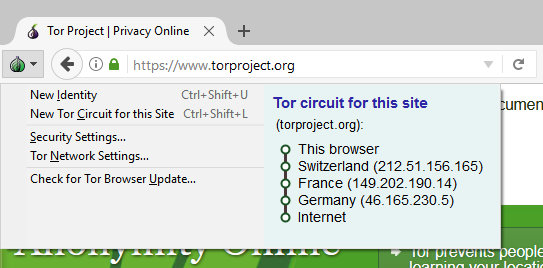
\includegraphics[width=\linewidth]{figures/tor-button-screenshot.jpg}
    \caption{A click on the onion icon reveals the Tor relays that constitute
    the circuit that was used to fetch the current page.  As of January 2018,
    the user interface is subject to a redesign~\cite{trac24309}.}
    \label{fig:tor-button}
\end{figure}

By clicking on the onion icon in the top left corner of Tor Browser (see
\Cref{fig:tor-button}), one can see the circuit that is used for the current web
site.  Some of our interviewees appreciated this visual feedback:

\begin{displayquote}[P08]
I love how I can monitor the network through this little kind of bar that comes
up.
\end{displayquote}

Not satisfied with seeing only the current circuit, some participants wished it
were easier to learn what else is happening behind the scenes:

\begin{displayquote}[P02]
{[It]} would be nice to have some kind of application, something on that browser,
that gives you an impression of\dots what the Tor Browser's actually doing.
\end{displayquote}

Finding the right balance between what information to show and what to hide is
challenging in itself and only exacerbated by Tor's heterogeneous user base.
While technical users may appreciate a look ``under the hood,'' non-technical
users, who often use Tor as a tool to get a specific job done, can easily feel
bewildered and overwhelmed.  One aspect, however, in which more transparency could
benefit Tor's entire user base is when web sites do not load, as suggested by
one participant:

\begin{displayquote}[P05]
\dots maybe some sort of graphical representation of is the circuit still
being built, or is the circuit built, and the site isn't responding at all to
the third relay?
\end{displayquote}

\subsubsection{Quantifying anonymity is hard}

The degree of anonymity that protects a Tor user in a given situation depends on
a number of variables including her guard relay, intermediate autonomous systems
on the network path, and other people that are using Tor at the same time, just
to name a few.  Unlike the \textsc{jap} anonymity tool~\cite{jap}, Tor Browser
makes no attempt to display the degree of anonymity it believes it can provide.
Asked about how well Tor works for them, one of our participants explained:

\begin{displayquote}[P12]
In terms of the anonymity, you can't really tell\dots That's fairly opaque, so I
can't even tell how effective that's working, or whether it is\dots
\end{displayquote}

Quantifying anonymity in a real-world setting is complex, error-prone, and often
misleading.  What is more, Tor Browser does not have available all the data it
needs to quantify its user's anonymity---an ``anonymity meter'' may therefore
create more problems than it solves.

\subsubsection{\textsc{ui}, speed, and \textsc{captcha}s remain frustrating}

Perhaps the most prevalent usability issue is, still, browsing speed.  An
interviewee provided the following anecdote:

\begin{displayquote}[P01]
The speed of it is problematic; sometimes I have a path that allows me to watch
full \textsc{hd} YouTube videos, and the next time, five minutes later, I'm
barely getting kilobytes through.
\end{displayquote}

Occasionally, Tor is preceded by its reputation, preparing users for what to
expect, as another interview participant reported:

\begin{displayquote}[P03]
I didn't think it was as slow as people say it was. People said it would be a
much slower experience but\ldots a little bit slower, but it didn't matter for
the things that I was doing.
\end{displayquote}

In addition to the perceived slowness, several participants lamented the
old-fashioned user interface, describing Tor Browser's looks as ``it felt like
it was about five years outdated,'' ``it looked like I was in 1982,'' and ``I
think the colors look a bit old fashioned and in the former Soviet Union.'' To
our surprise, one participant expressed that the antiquated user interface also
evoked trust:

\begin{displayquote}[P02]
At the same time I thought\ldots it gave them a certain amount of credibility,
like they weren't building this for the looks, but they were building it for
functionality\ldots  At the same time, as I thought it was outdated in terms of
how it looked, I also thought it was sort of genuine in a way.
\end{displayquote}

Orthogonal to Tor's speed and user interface, the browsing experience
occasionally suffers.  Relying on naive, \textsc{ip} address-based metrics of
``maliciousness,'' some content delivery networks such as Cloudflare label Tor
exit relays as malicious which results in Tor users' having to solve (sometimes
multiple) \textsc{captcha}s before being granted access to a web site.  In 2016,
Khattak \ea\ documented the issue for a number of content
providers~\cite{Khattak2016a}.  Both survey and interview participants brought
up the topic and one person managed to depict the issue without the use of
profanity:

\begin{displayquote}[P06]
It is still sometimes challenging using some everyday services because of
\textsc{captcha}s and those things, but I also understand that's not so much to
do with Tor, but to do with the creators of those web sites.
\end{displayquote}

\subsubsection{Empowerment through security and privacy}

It comes as no surprise that our data reveals that the main benefit of Tor
Browser is the increase in privacy and security, brought up by practically all
of our interview participants.  One of our more technical interviewees (and
several of our survey respondents) further distinguished between security and
privacy.  Asked about if they feel safer when using Tor, they responded:

\begin{displayquote}[P06]
In a privacy sense, I do. In a security sense\ldots I don't assume that Tor is
protecting me from all of the vulnerabilities or exploits that I might
encounter\ldots
\end{displayquote}

Besides the obvious improvement in security and privacy, a defining aspect of
Tor is that it puts users back in control, or, as one of our participants
eloquently phrased it:

\begin{displayquote}[P02]
I feel like I'm more in control of my internet experience that way, I'm not sort
of like a will-less victim of what other people want to do with me, so I feel
I'm more empowered and have more agency when I use the Tor Browser.
\end{displayquote}

\subsection{Onion service usage}

We now move on to results specific to onion services, the focus of our online
survey.  The usage frequency of onion services is almost uniformly distributed
among our respondents; 24\% use onion sites less than once a month, 22\% use
them about monthly, 25\% weekly, and 23\% daily.  The remaining 6\% has never
used an onion service before.

The majority of our respondents (61.8\%) have used onion services for purposes
other than web browsing before.  Several protocols, such as the chat application
Ricochet~\cite{ricochet} and the file sharing application
OnionShare~\cite{onionshare}, were purpose-built on top of onion services while
existing \textsc{tcp}-based tools, such as \textsc{ssh}, can transparently use
onion addresses instead of traditional \textsc{ip} addresses.  Almost one third
(29.7\%) of our participants use onion services for non-browsing activities at
least once a week.

But why do Tor users browse onion services in the first place?
\Cref{fig:onion-usage} provides some insight.  The majority uses onion services
because of the additional anonymity (70\%) and the additional security (61\%).
For 46\% it is the only way to access content they enjoy, making the use of
onion services a necessity.  27\% of our respondents found themselves eager to
learn more about the ``Dark Web'' and set out to satisfy their curiosity while
19\% occasionally stumble upon links to onion services in their day-to-day
browsing activity.  Respondents who selected ``Other'' gave a variety of
reasons, the most predominant being the ability to set up a \textsc{tcp} service
behind a \textsc{nat} device.  That makes it possible to run an \textsc{ssh}
server in a home network that has neither a permanent \textsc{ip} address nor
port forwarding.  Others use onion services to reduce the load on exit relays,
to do technical research, and to access sites that are otherwise unavailable.

\begin{figure}[t]
    \centering
    % Created by tikzDevice version 0.10.1 on 2018-01-12 16:14:57
% !TEX encoding = UTF-8 Unicode
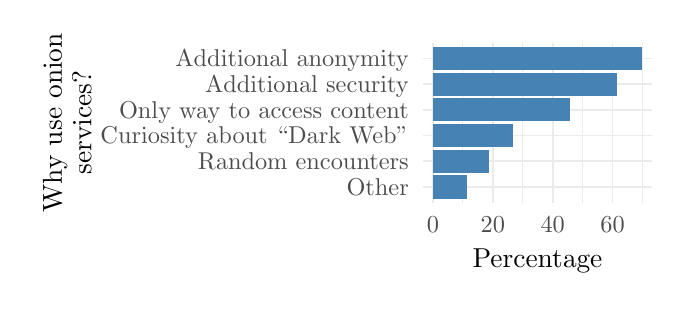
\begin{tikzpicture}[x=1pt,y=1pt]
\definecolor{fillColor}{RGB}{255,255,255}
\path[use as bounding box,fill=fillColor,fill opacity=0.00] (0,0) rectangle (231.26, 93.95);
\begin{scope}
\path[clip] (142.68, 30.77) rectangle (225.76, 88.45);
\definecolor{drawColor}{gray}{0.92}

\path[draw=drawColor,line width= 0.3pt,line join=round] (157.27, 30.77) --
	(157.27, 88.45);

\path[draw=drawColor,line width= 0.3pt,line join=round] (178.90, 30.77) --
	(178.90, 88.45);

\path[draw=drawColor,line width= 0.3pt,line join=round] (200.54, 30.77) --
	(200.54, 88.45);

\path[draw=drawColor,line width= 0.3pt,line join=round] (222.17, 30.77) --
	(222.17, 88.45);

\path[draw=drawColor,line width= 0.6pt,line join=round] (142.68, 36.35) --
	(225.76, 36.35);

\path[draw=drawColor,line width= 0.6pt,line join=round] (142.68, 45.66) --
	(225.76, 45.66);

\path[draw=drawColor,line width= 0.6pt,line join=round] (142.68, 54.96) --
	(225.76, 54.96);

\path[draw=drawColor,line width= 0.6pt,line join=round] (142.68, 64.26) --
	(225.76, 64.26);

\path[draw=drawColor,line width= 0.6pt,line join=round] (142.68, 73.57) --
	(225.76, 73.57);

\path[draw=drawColor,line width= 0.6pt,line join=round] (142.68, 82.87) --
	(225.76, 82.87);

\path[draw=drawColor,line width= 0.6pt,line join=round] (146.45, 30.77) --
	(146.45, 88.45);

\path[draw=drawColor,line width= 0.6pt,line join=round] (168.09, 30.77) --
	(168.09, 88.45);

\path[draw=drawColor,line width= 0.6pt,line join=round] (189.72, 30.77) --
	(189.72, 88.45);

\path[draw=drawColor,line width= 0.6pt,line join=round] (211.35, 30.77) --
	(211.35, 88.45);
\definecolor{fillColor}{RGB}{70,130,180}

\path[fill=fillColor] (146.45, 32.17) rectangle (158.77, 40.54);

\path[fill=fillColor] (146.45, 41.47) rectangle (166.57, 49.84);

\path[fill=fillColor] (146.45, 50.77) rectangle (175.40, 59.15);

\path[fill=fillColor] (146.45, 60.08) rectangle (196.12, 68.45);

\path[fill=fillColor] (146.45, 69.38) rectangle (212.96, 77.75);

\path[fill=fillColor] (146.45, 78.68) rectangle (221.99, 87.06);
\end{scope}
\begin{scope}
\path[clip] (  0.00,  0.00) rectangle (231.26, 93.95);
\definecolor{drawColor}{gray}{0.30}

\node[text=drawColor,anchor=base east,inner sep=0pt, outer sep=0pt, scale=  0.88] at (137.73, 33.32) {Other};

\node[text=drawColor,anchor=base east,inner sep=0pt, outer sep=0pt, scale=  0.88] at (137.73, 42.63) {Random encounters};

\node[text=drawColor,anchor=base east,inner sep=0pt, outer sep=0pt, scale=  0.88] at (137.73, 51.93) {Curiosity about ``Dark Web''};

\node[text=drawColor,anchor=base east,inner sep=0pt, outer sep=0pt, scale=  0.88] at (137.73, 61.23) {Only way to access content};

\node[text=drawColor,anchor=base east,inner sep=0pt, outer sep=0pt, scale=  0.88] at (137.73, 70.54) {Additional security};

\node[text=drawColor,anchor=base east,inner sep=0pt, outer sep=0pt, scale=  0.88] at (137.73, 79.84) {Additional anonymity};
\end{scope}
\begin{scope}
\path[clip] (  0.00,  0.00) rectangle (231.26, 93.95);
\definecolor{drawColor}{gray}{0.30}

\node[text=drawColor,anchor=base,inner sep=0pt, outer sep=0pt, scale=  0.88] at (146.45, 19.76) {0};

\node[text=drawColor,anchor=base,inner sep=0pt, outer sep=0pt, scale=  0.88] at (168.09, 19.76) {20};

\node[text=drawColor,anchor=base,inner sep=0pt, outer sep=0pt, scale=  0.88] at (189.72, 19.76) {40};

\node[text=drawColor,anchor=base,inner sep=0pt, outer sep=0pt, scale=  0.88] at (211.35, 19.76) {60};
\end{scope}
\begin{scope}
\path[clip] (  0.00,  0.00) rectangle (231.26, 93.95);
\definecolor{drawColor}{RGB}{0,0,0}

\node[text=drawColor,anchor=base,inner sep=0pt, outer sep=0pt, scale=  0.99] at (184.22,  7.44) {Percentage};
\end{scope}
\begin{scope}
\path[clip] (  0.00,  0.00) rectangle (231.26, 93.95);
\definecolor{drawColor}{RGB}{0,0,0}

\node[text=drawColor,rotate= 90.00,anchor=base,inner sep=0pt, outer sep=0pt, scale=  0.99] at ( 12.32, 59.61) {Why use onion};

\node[text=drawColor,rotate= 90.00,anchor=base,inner sep=0pt, outer sep=0pt, scale=  0.99] at ( 23.01, 59.61) {services?};
\end{scope}
\end{tikzpicture}

    \caption{Our respondents' (multiple choice) reasons for using onion
    services.}
    \label{fig:onion-usage}
\end{figure}

\subsubsection{Mental models are often patchy}
\label{sec:mental-models}

Recall that we asked our interview participants to draw sketches of Tor and
onion services.\footnote{All sketches are available online at
\url{https://nymity.ch/onion-services/mental-models/}.}   Everybody drew a
sketch of Tor but some did not draw onion services because they had not
experienced them.  Interestingly, all participants understood that key to Tor's
anonymity is the bouncing of network traffic across several relays, as evidenced
by \Cref{fig:tor-sketch}, drawn by a participant with no technical
background.\footnote{However, the sketch got two details wrong: the number of
hops in a Tor circuit is three, and the circuit's forward and reverse path are
identical.} Analogously, most of our participants understood that network
traffic does not leave the Tor network when connecting to onion services.
\Cref{fig:os-sketch} illustrates an example, again drawn by a non-technical
participant.  The last hop in the circuit is an onion, correctly suggesting that
network traffic does not leave the Tor network.

\begin{figure}[t]
    \centering

    \begin{subfigure}[t]{\linewidth}
        \centering
        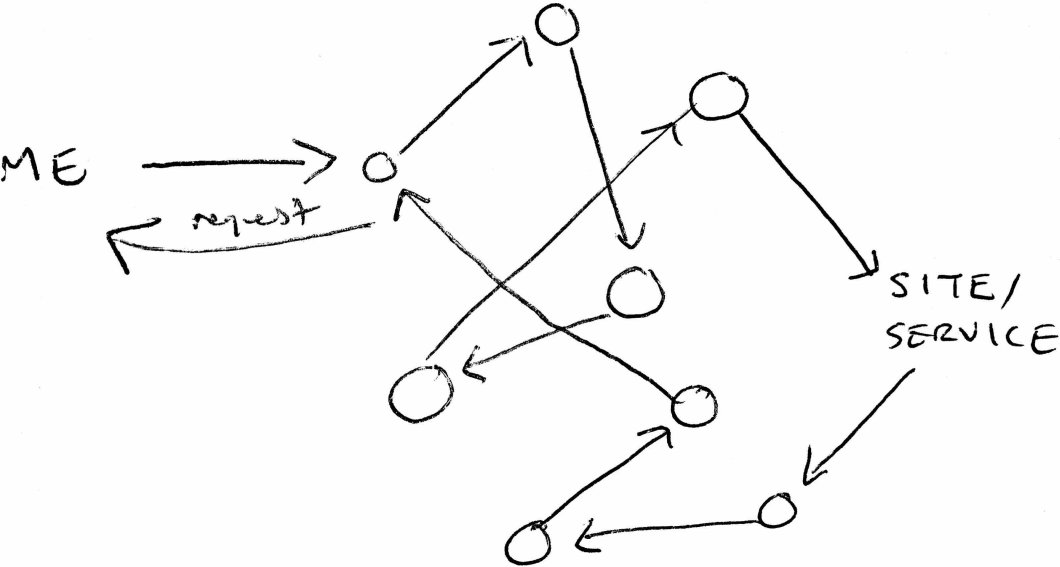
\includegraphics[width=0.8\linewidth]{figures/tor-sketch.jpg}
        \subcaption{A non-technical interview subject's (P08) sketch of how they
        believe Tor works.  The participant correctly understands the concept of
        bouncing network traffic over several hops.}
        \label{fig:tor-sketch}
    \end{subfigure}

    \begin{subfigure}[t]{\linewidth}
        \centering
        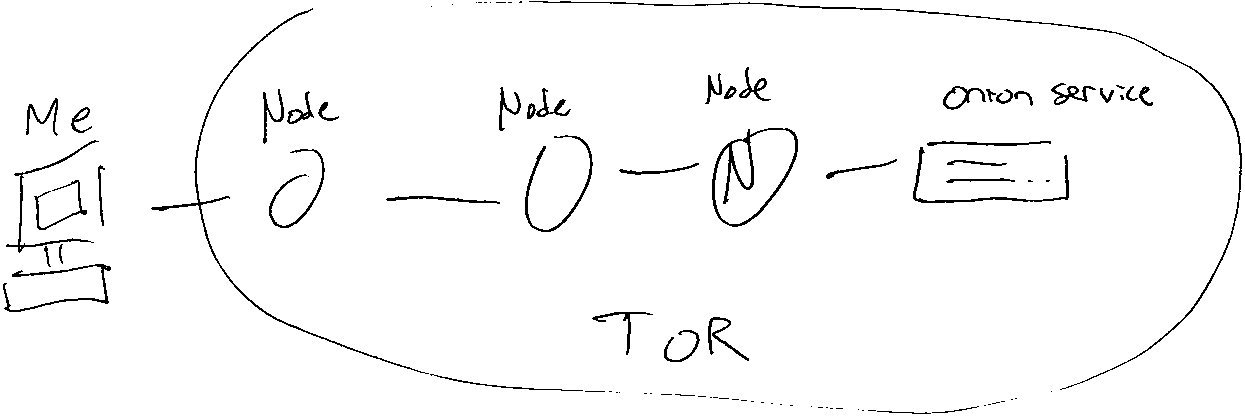
\includegraphics[width=0.8\linewidth]{figures/os-sketch.jpg}
        \subcaption{A technical interview subject's (P01) sketch of their mental
        model of an onion service.  Instead of a web site, the final hop is
        another Tor hop.}
        \label{fig:os-sketch}
    \end{subfigure}

    \caption{Sketches of two different, non-technical interview participants of
    how Tor works (top) and how onion services work (bottom).}
\end{figure}

Some of our interviewees did not distinguish disguising their \textsc{ip}
address from disguising their real-world identity and instead used the umbrella
term of ``anonymity'' to refer to both concepts.  This conflation of concepts
paints an incomplete picture of the security and privacy guarantees that Tor
provides, further illustrated by one participant's question:

\begin{displayquote}[P07]
What's the point of going to Facebook using onion services when their business
model is still about collecting your data?
\end{displayquote}

There is merit in using Facebook's onion service.  While the company indeed
knows who is logging in, it does not know Tor users' \textsc{ip} address (and
hence location) or operating system.  On top of that, onion services provide
end-to-end security and self-authenticating names.  These benefits are difficult
to convey to non-technical users, and even experts sometimes advocate an ``all or
nothing'' approach to online anonymity, overlooking important nuances.

An unrelated, yet hardly unexpected, flawed mental model is the domain format of
onion services.  Some users have come to believe that the seemingly-random
characters in onion domains are the reason why onion services are anonymous.
Accordingly, these users also believe that vanity domains are ``less anonymous''
because part of their domains is clearly not random.

\subsubsection{Makeshift solutions ease onion service discovery}

Recall that a freshly set up onion service is private by default, leaving it up
to its operator to disseminate the domain.  Established search engines such as
Google are therefore inadequate to find content on onion services.  We wanted to
find out how our respondents discover onion services.
\Cref{fig:onion-discovery} illustrates the results.  The three most popular ways
of discovering new onion sites, all approximating 50\%, are \first~social
networking sites such as Twitter and Reddit, \second~the list of search engines
such as Ahmia\footnote{Ahmia.fi is an onion site search engine that crawls
user-submitted onion domains.  It publishes the list of all indexed onion
services at \url{https://ahmia.fi/onions/}.}, and \third~randomly encountering
links when browsing the web.

While significantly less popular, discovering onion domains through friends and
family has the advantage that domains come from a trusted source---an aspect
that mattered to some of our survey and interview participants.  Finally, a mere
4\% indicated that they are not interested in learning about new onion services.

Respondents who selected ``Other'' predominantly brought up
independently-maintained lists of onion services and aggregators.  A noteworthy
example is the Hidden Wiki, a community-curated and frequently-forked wiki that
contains categorized links to onion services.

\begin{figure}[t]
    \centering
    % Created by tikzDevice version 0.10.1 on 2018-01-12 16:15:03
% !TEX encoding = UTF-8 Unicode
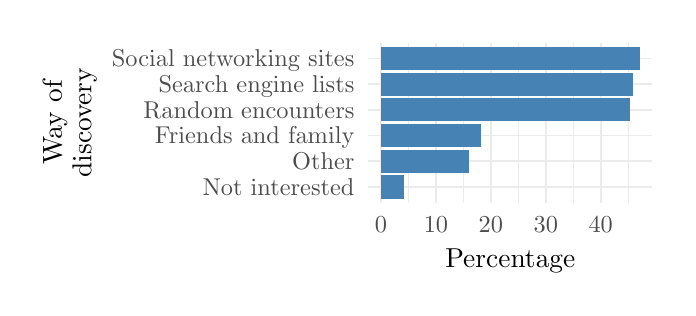
\begin{tikzpicture}[x=1pt,y=1pt]
\definecolor{fillColor}{RGB}{255,255,255}
\path[use as bounding box,fill=fillColor,fill opacity=0.00] (0,0) rectangle (231.26, 93.95);
\begin{scope}
\path[clip] (123.02, 30.77) rectangle (225.76, 88.45);
\definecolor{drawColor}{gray}{0.92}

\path[draw=drawColor,line width= 0.3pt,line join=round] (137.61, 30.77) --
	(137.61, 88.45);

\path[draw=drawColor,line width= 0.3pt,line join=round] (157.46, 30.77) --
	(157.46, 88.45);

\path[draw=drawColor,line width= 0.3pt,line join=round] (177.31, 30.77) --
	(177.31, 88.45);

\path[draw=drawColor,line width= 0.3pt,line join=round] (197.16, 30.77) --
	(197.16, 88.45);

\path[draw=drawColor,line width= 0.3pt,line join=round] (217.00, 30.77) --
	(217.00, 88.45);

\path[draw=drawColor,line width= 0.6pt,line join=round] (123.02, 36.35) --
	(225.76, 36.35);

\path[draw=drawColor,line width= 0.6pt,line join=round] (123.02, 45.66) --
	(225.76, 45.66);

\path[draw=drawColor,line width= 0.6pt,line join=round] (123.02, 54.96) --
	(225.76, 54.96);

\path[draw=drawColor,line width= 0.6pt,line join=round] (123.02, 64.26) --
	(225.76, 64.26);

\path[draw=drawColor,line width= 0.6pt,line join=round] (123.02, 73.57) --
	(225.76, 73.57);

\path[draw=drawColor,line width= 0.6pt,line join=round] (123.02, 82.87) --
	(225.76, 82.87);

\path[draw=drawColor,line width= 0.6pt,line join=round] (127.69, 30.77) --
	(127.69, 88.45);

\path[draw=drawColor,line width= 0.6pt,line join=round] (147.54, 30.77) --
	(147.54, 88.45);

\path[draw=drawColor,line width= 0.6pt,line join=round] (167.38, 30.77) --
	(167.38, 88.45);

\path[draw=drawColor,line width= 0.6pt,line join=round] (187.23, 30.77) --
	(187.23, 88.45);

\path[draw=drawColor,line width= 0.6pt,line join=round] (207.08, 30.77) --
	(207.08, 88.45);
\definecolor{fillColor}{RGB}{70,130,180}

\path[fill=fillColor] (127.69, 32.17) rectangle (135.96, 40.54);

\path[fill=fillColor] (127.69, 41.47) rectangle (159.33, 49.84);

\path[fill=fillColor] (127.69, 50.77) rectangle (163.85, 59.15);

\path[fill=fillColor] (127.69, 60.08) rectangle (217.70, 68.45);

\path[fill=fillColor] (127.69, 69.38) rectangle (218.83, 77.75);

\path[fill=fillColor] (127.69, 78.68) rectangle (221.09, 87.06);
\end{scope}
\begin{scope}
\path[clip] (  0.00,  0.00) rectangle (231.26, 93.95);
\definecolor{drawColor}{gray}{0.30}

\node[text=drawColor,anchor=base east,inner sep=0pt, outer sep=0pt, scale=  0.88] at (118.07, 33.32) {Not interested};

\node[text=drawColor,anchor=base east,inner sep=0pt, outer sep=0pt, scale=  0.88] at (118.07, 42.63) {Other};

\node[text=drawColor,anchor=base east,inner sep=0pt, outer sep=0pt, scale=  0.88] at (118.07, 51.93) {Friends and family};

\node[text=drawColor,anchor=base east,inner sep=0pt, outer sep=0pt, scale=  0.88] at (118.07, 61.23) {Random encounters};

\node[text=drawColor,anchor=base east,inner sep=0pt, outer sep=0pt, scale=  0.88] at (118.07, 70.54) {Search engine lists};

\node[text=drawColor,anchor=base east,inner sep=0pt, outer sep=0pt, scale=  0.88] at (118.07, 79.84) {Social networking sites};
\end{scope}
\begin{scope}
\path[clip] (  0.00,  0.00) rectangle (231.26, 93.95);
\definecolor{drawColor}{gray}{0.30}

\node[text=drawColor,anchor=base,inner sep=0pt, outer sep=0pt, scale=  0.88] at (127.69, 19.76) {0};

\node[text=drawColor,anchor=base,inner sep=0pt, outer sep=0pt, scale=  0.88] at (147.54, 19.76) {10};

\node[text=drawColor,anchor=base,inner sep=0pt, outer sep=0pt, scale=  0.88] at (167.38, 19.76) {20};

\node[text=drawColor,anchor=base,inner sep=0pt, outer sep=0pt, scale=  0.88] at (187.23, 19.76) {30};

\node[text=drawColor,anchor=base,inner sep=0pt, outer sep=0pt, scale=  0.88] at (207.08, 19.76) {40};
\end{scope}
\begin{scope}
\path[clip] (  0.00,  0.00) rectangle (231.26, 93.95);
\definecolor{drawColor}{RGB}{0,0,0}

\node[text=drawColor,anchor=base,inner sep=0pt, outer sep=0pt, scale=  0.99] at (174.39,  7.44) {Percentage};
\end{scope}
\begin{scope}
\path[clip] (  0.00,  0.00) rectangle (231.26, 93.95);
\definecolor{drawColor}{RGB}{0,0,0}

\node[text=drawColor,rotate= 90.00,anchor=base,inner sep=0pt, outer sep=0pt, scale=  0.99] at ( 12.32, 59.61) {Way of};

\node[text=drawColor,rotate= 90.00,anchor=base,inner sep=0pt, outer sep=0pt, scale=  0.99] at ( 23.01, 59.61) {discovery};
\end{scope}
\end{tikzpicture}

    \caption{Our respondents' (multiple choice) methods of discovering onion
    services.}
    \label{fig:onion-discovery}
\end{figure}

The next question in our survey asked if our respondents are satisfied with the
way they discover onion services.  60\% selected ``Yes'' while 40\% selected
``No.'' Some respondents who selected ``Yes'' brought up that they have no
interest in learning about new onion services, in part because they only use a
small set of onion services.  Among the people who are not satisfied, the most
prominent complaint was about broken links on onion site lists.  There is
non-trivial churn among onion sites, and our respondents were frustrated that
existing lists are typically not curated and link to numerous dead domains.  The
lack of curation also leads to these lists' containing the occasional scam and
phishing site.  The difficulty of telling apart two given onion domain names
exacerbates this issue for users.  Another common wish for aggregators was for
them to be more verbose in their description of onion sites.  In particular,
some respondents want to avoid illegal and pornographic content, which is often
difficult if the description is vague and the onion domain reveals nothing about
its content.  Many respondents were not aware of search engines such as Ahmia.
Among those that were, many were dissatisfied with both the search results and
the number of indexed onion sites.  Unsurprisingly, a ``Google for onion sites''
was a frequent wish.

Many respondents expressed frustration about the difficulty of finding out if
example.com has a corresponding onion service.  A common wish was to have
example.com list its onion service prominently in a footer.  Ironically, some
respondents were surprised that torproject.org has a corresponding onion
site---they could not find it on the web site.  Interestingly, some respondents
voiced frustration about various usability issues but mentioned in the same
sentence that this is an inherent trade-off of privacy technology, suggesting
that there is nothing that can be done about it.

\subsubsection{Onion domain management is problematic}

Conventional domains are designed to be easy to remember and recognize.  But how
do users handle randomly-generated onion domains?  Our survey
\hyperref[q3_7]{question 3.7} sought an answer, and the results are illustrated
in \Cref{fig:onion-domain-mgmt}.

\begin{figure}[t]
    \centering
    % Created by tikzDevice version 0.10.1 on 2018-02-09 14:36:33
% !TEX encoding = UTF-8 Unicode
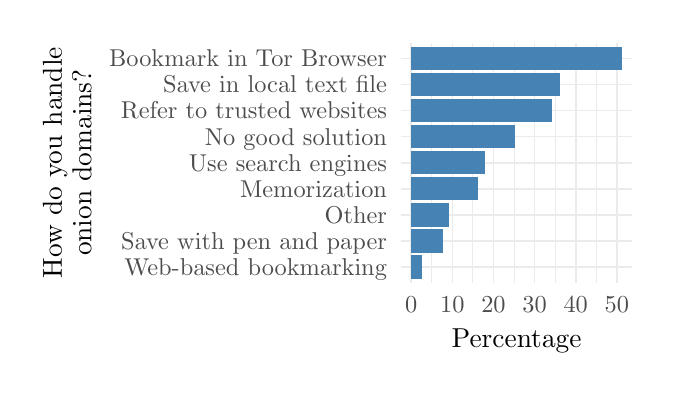
\begin{tikzpicture}[x=1pt,y=1pt]
\definecolor{fillColor}{RGB}{255,255,255}
\path[use as bounding box,fill=fillColor,fill opacity=0.00] (0,0) rectangle (224.04,122.86);
\begin{scope}
\path[clip] (134.78, 30.77) rectangle (218.54,117.36);
\definecolor{drawColor}{gray}{0.92}

\path[draw=drawColor,line width= 0.3pt,line join=round] (146.02, 30.77) --
	(146.02,117.36);

\path[draw=drawColor,line width= 0.3pt,line join=round] (160.88, 30.77) --
	(160.88,117.36);

\path[draw=drawColor,line width= 0.3pt,line join=round] (175.74, 30.77) --
	(175.74,117.36);

\path[draw=drawColor,line width= 0.3pt,line join=round] (190.61, 30.77) --
	(190.61,117.36);

\path[draw=drawColor,line width= 0.3pt,line join=round] (205.47, 30.77) --
	(205.47,117.36);

\path[draw=drawColor,line width= 0.6pt,line join=round] (134.78, 36.42) --
	(218.54, 36.42);

\path[draw=drawColor,line width= 0.6pt,line join=round] (134.78, 45.83) --
	(218.54, 45.83);

\path[draw=drawColor,line width= 0.6pt,line join=round] (134.78, 55.24) --
	(218.54, 55.24);

\path[draw=drawColor,line width= 0.6pt,line join=round] (134.78, 64.65) --
	(218.54, 64.65);

\path[draw=drawColor,line width= 0.6pt,line join=round] (134.78, 74.07) --
	(218.54, 74.07);

\path[draw=drawColor,line width= 0.6pt,line join=round] (134.78, 83.48) --
	(218.54, 83.48);

\path[draw=drawColor,line width= 0.6pt,line join=round] (134.78, 92.89) --
	(218.54, 92.89);

\path[draw=drawColor,line width= 0.6pt,line join=round] (134.78,102.30) --
	(218.54,102.30);

\path[draw=drawColor,line width= 0.6pt,line join=round] (134.78,111.71) --
	(218.54,111.71);

\path[draw=drawColor,line width= 0.6pt,line join=round] (138.58, 30.77) --
	(138.58,117.36);

\path[draw=drawColor,line width= 0.6pt,line join=round] (153.45, 30.77) --
	(153.45,117.36);

\path[draw=drawColor,line width= 0.6pt,line join=round] (168.31, 30.77) --
	(168.31,117.36);

\path[draw=drawColor,line width= 0.6pt,line join=round] (183.17, 30.77) --
	(183.17,117.36);

\path[draw=drawColor,line width= 0.6pt,line join=round] (198.04, 30.77) --
	(198.04,117.36);

\path[draw=drawColor,line width= 0.6pt,line join=round] (212.90, 30.77) --
	(212.90,117.36);
\definecolor{fillColor}{RGB}{70,130,180}

\path[fill=fillColor] (138.58, 32.18) rectangle (142.54, 40.66);

\path[fill=fillColor] (138.58, 41.60) rectangle (150.15, 50.07);

\path[fill=fillColor] (138.58, 51.01) rectangle (152.13, 59.48);

\path[fill=fillColor] (138.58, 60.42) rectangle (162.84, 68.89);

\path[fill=fillColor] (138.58, 69.83) rectangle (165.10, 78.30);

\path[fill=fillColor] (138.58, 79.24) rectangle (176.10, 87.71);

\path[fill=fillColor] (138.58, 88.65) rectangle (189.36, 97.12);

\path[fill=fillColor] (138.58, 98.07) rectangle (192.45,106.54);

\path[fill=fillColor] (138.58,107.48) rectangle (214.73,115.95);
\end{scope}
\begin{scope}
\path[clip] (  0.00,  0.00) rectangle (224.04,122.86);
\definecolor{drawColor}{gray}{0.30}

\node[text=drawColor,anchor=base east,inner sep=0pt, outer sep=0pt, scale=  0.88] at (129.83, 33.39) {Web-based bookmarking};

\node[text=drawColor,anchor=base east,inner sep=0pt, outer sep=0pt, scale=  0.88] at (129.83, 42.80) {Save with pen and paper};

\node[text=drawColor,anchor=base east,inner sep=0pt, outer sep=0pt, scale=  0.88] at (129.83, 52.21) {Other};

\node[text=drawColor,anchor=base east,inner sep=0pt, outer sep=0pt, scale=  0.88] at (129.83, 61.62) {Memorization};

\node[text=drawColor,anchor=base east,inner sep=0pt, outer sep=0pt, scale=  0.88] at (129.83, 71.04) {Use search engines};

\node[text=drawColor,anchor=base east,inner sep=0pt, outer sep=0pt, scale=  0.88] at (129.83, 80.45) {No good solution};

\node[text=drawColor,anchor=base east,inner sep=0pt, outer sep=0pt, scale=  0.88] at (129.83, 89.86) {Refer to trusted websites};

\node[text=drawColor,anchor=base east,inner sep=0pt, outer sep=0pt, scale=  0.88] at (129.83, 99.27) {Save in local text file};

\node[text=drawColor,anchor=base east,inner sep=0pt, outer sep=0pt, scale=  0.88] at (129.83,108.68) {Bookmark in Tor Browser};
\end{scope}
\begin{scope}
\path[clip] (  0.00,  0.00) rectangle (224.04,122.86);
\definecolor{drawColor}{gray}{0.30}

\node[text=drawColor,anchor=base,inner sep=0pt, outer sep=0pt, scale=  0.88] at (138.58, 19.76) {0};

\node[text=drawColor,anchor=base,inner sep=0pt, outer sep=0pt, scale=  0.88] at (153.45, 19.76) {10};

\node[text=drawColor,anchor=base,inner sep=0pt, outer sep=0pt, scale=  0.88] at (168.31, 19.76) {20};

\node[text=drawColor,anchor=base,inner sep=0pt, outer sep=0pt, scale=  0.88] at (183.17, 19.76) {30};

\node[text=drawColor,anchor=base,inner sep=0pt, outer sep=0pt, scale=  0.88] at (198.04, 19.76) {40};

\node[text=drawColor,anchor=base,inner sep=0pt, outer sep=0pt, scale=  0.88] at (212.90, 19.76) {50};
\end{scope}
\begin{scope}
\path[clip] (  0.00,  0.00) rectangle (224.04,122.86);
\definecolor{drawColor}{RGB}{0,0,0}

\node[text=drawColor,anchor=base,inner sep=0pt, outer sep=0pt, scale=  0.99] at (176.66,  7.44) {Percentage};
\end{scope}
\begin{scope}
\path[clip] (  0.00,  0.00) rectangle (224.04,122.86);
\definecolor{drawColor}{RGB}{0,0,0}

\node[text=drawColor,rotate= 90.00,anchor=base,inner sep=0pt, outer sep=0pt, scale=  0.99] at ( 12.32, 74.07) {How do you handle};

\node[text=drawColor,rotate= 90.00,anchor=base,inner sep=0pt, outer sep=0pt, scale=  0.99] at ( 23.01, 74.07) {onion domains?};
\end{scope}
\end{tikzpicture}

    \caption{The strategies that our respondents use to handle onion domains.
    More than half use bookmarks inside of Tor Browser and a quarter thinks that
    there is no good solution.}
    \label{fig:onion-domain-mgmt}
\end{figure}

Most respondents use Tor Browser's bookmarks to save onion domains.  While
convenient, it leaves a trace of (presumably) visited sites on somebody's
computer.  One of Tor Browser's security requirements is ``disk avoidance,''
\ie, the browser must not write anything to disk that would reveal the user's
browsing history~\cite[\S~2.1]{Perry2017a}.  Bookmarking links is a violation of
this security requirement albeit requested by the user.  Many of our respondents
were aware of this issue, and about a dozen respondents who selected ``Other''
stated that they store onion domains in an encrypted manner---either in a text
file or in their password manager.  Somewhat less popular is saving onion
domains in local text files (36\%), getting them from trusted web sites (34\%),
using search engines (18\%), memorizing domains (16\%), using some other
techniques (9\%), or employing pen and paper (8\%).  Notably, one quarter of our
respondents do not have a good solution to the problem.  Given the alarming
number of (possibly insecure) home-baked solutions, a Tor Browser extension that
solves this problem may be warranted.

Of the respondents who memorize onion domains, we found that most respondents
memorize either one onion domain (15\% of total respondents) or four onion
domains (11\% of total respondents); significantly fewer respondents memorize
two domains (5\%), three domains (4\%), and more than four domains (1\%).  As
mentioned above, bookmarking onion domains leaves a trace, and about 28\% of
respondents said they memorize onion domains to prevent this digital trace.  On
the other hand, more respondents memorize domains \first~to allow them to open
the site more quickly (51\%), \second~to ensure that they are visiting the
correct site and not a phishing site (44\%), and \third~automatically start to
memorize domains because of typing it many times (60\%).

Our survey also asked respondents about whether or not they memorize vanity
domains---specifically facebookcorewwwi.onion---and how difficult they find it
to memorize onion domains of differing levels of vanity.  59\% of respondents
replied that facebookcorewwwi.onion is among the sites that they have memorized.
This is because it is ``easy to memorize'' and ``after seeing [it] many times, I
automatically start to memorize it.''  When asked about different levels of
vanity domains, the respondents expressed differing levels of ease for 
memorizing them; these results are shown in \Cref{fig:memorize-domains}.
\textsc{url}s such as expyuzz4wqqyqhjn.onion and torproz4wqqyqhjn.onion are
harder for respondents to remember because they mention that ``numbers make the
names harder to remember.''  Other respondents stated that domains are easier to
remember when they can be pronounced.  One respondent described it saying
``phonetic pronunciation plays a large part in how I remember onions.'' Many
other respondents stated that onion domains that are supported by a mnemonic are
also easier to remember.  

\begin{figure}[t]
    \centering
    % Created by tikzDevice version 0.10.1 on 2018-02-09 14:43:10
% !TEX encoding = UTF-8 Unicode
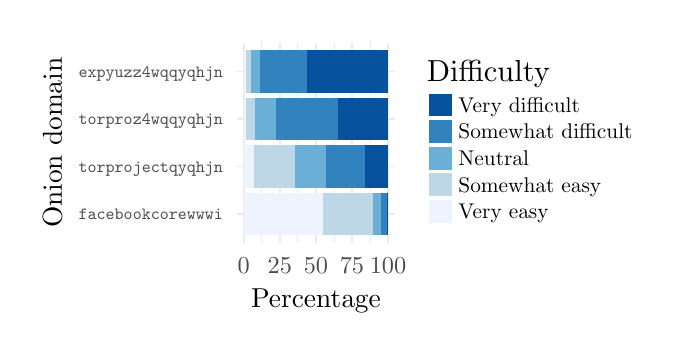
\begin{tikzpicture}[x=1pt,y=1pt]
\definecolor{fillColor}{RGB}{255,255,255}
\path[use as bounding box,fill=fillColor,fill opacity=0.00] (0,0) rectangle (224.04,108.41);
\begin{scope}
\path[clip] ( 75.47, 30.77) rectangle (132.84,102.91);
\definecolor{drawColor}{gray}{0.92}

\path[draw=drawColor,line width= 0.3pt,line join=round] ( 84.60, 30.77) --
	( 84.60,102.91);

\path[draw=drawColor,line width= 0.3pt,line join=round] ( 97.64, 30.77) --
	( 97.64,102.91);

\path[draw=drawColor,line width= 0.3pt,line join=round] (110.67, 30.77) --
	(110.67,102.91);

\path[draw=drawColor,line width= 0.3pt,line join=round] (123.71, 30.77) --
	(123.71,102.91);

\path[draw=drawColor,line width= 0.6pt,line join=round] ( 75.47, 41.08) --
	(132.84, 41.08);

\path[draw=drawColor,line width= 0.6pt,line join=round] ( 75.47, 58.25) --
	(132.84, 58.25);

\path[draw=drawColor,line width= 0.6pt,line join=round] ( 75.47, 75.43) --
	(132.84, 75.43);

\path[draw=drawColor,line width= 0.6pt,line join=round] ( 75.47, 92.60) --
	(132.84, 92.60);

\path[draw=drawColor,line width= 0.6pt,line join=round] ( 78.08, 30.77) --
	( 78.08,102.91);

\path[draw=drawColor,line width= 0.6pt,line join=round] ( 91.12, 30.77) --
	( 91.12,102.91);

\path[draw=drawColor,line width= 0.6pt,line join=round] (104.16, 30.77) --
	(104.16,102.91);

\path[draw=drawColor,line width= 0.6pt,line join=round] (117.19, 30.77) --
	(117.19,102.91);

\path[draw=drawColor,line width= 0.6pt,line join=round] (130.23, 30.77) --
	(130.23,102.91);
\definecolor{fillColor}{RGB}{239,243,255}

\path[fill=fillColor] ( 78.08, 33.35) rectangle (106.78, 48.81);
\definecolor{fillColor}{RGB}{189,215,231}

\path[fill=fillColor] (106.78, 33.35) rectangle (124.77, 48.81);
\definecolor{fillColor}{RGB}{107,174,214}

\path[fill=fillColor] (124.77, 33.35) rectangle (127.56, 48.81);
\definecolor{fillColor}{RGB}{49,130,189}

\path[fill=fillColor] (127.56, 33.35) rectangle (129.70, 48.81);
\definecolor{fillColor}{RGB}{8,81,156}

\path[fill=fillColor] (129.70, 33.35) rectangle (130.24, 48.81);
\definecolor{fillColor}{RGB}{239,243,255}

\path[fill=fillColor] ( 78.08, 50.52) rectangle ( 81.93, 65.98);
\definecolor{fillColor}{RGB}{189,215,231}

\path[fill=fillColor] ( 81.93, 50.52) rectangle ( 96.50, 65.98);
\definecolor{fillColor}{RGB}{107,174,214}

\path[fill=fillColor] ( 96.50, 50.52) rectangle (107.64, 65.98);
\definecolor{fillColor}{RGB}{49,130,189}

\path[fill=fillColor] (107.64, 50.52) rectangle (121.88, 65.98);
\definecolor{fillColor}{RGB}{8,81,156}

\path[fill=fillColor] (121.88, 50.52) rectangle (130.24, 65.98);
\definecolor{fillColor}{RGB}{239,243,255}

\path[fill=fillColor] ( 78.08, 67.70) rectangle ( 78.94, 83.15);
\definecolor{fillColor}{RGB}{189,215,231}

\path[fill=fillColor] ( 78.94, 67.70) rectangle ( 82.05, 83.15);
\definecolor{fillColor}{RGB}{107,174,214}

\path[fill=fillColor] ( 82.05, 67.70) rectangle ( 89.67, 83.15);
\definecolor{fillColor}{RGB}{49,130,189}

\path[fill=fillColor] ( 89.67, 67.70) rectangle (112.21, 83.15);
\definecolor{fillColor}{RGB}{8,81,156}

\path[fill=fillColor] (112.21, 67.70) rectangle (130.24, 83.15);
\definecolor{fillColor}{RGB}{239,243,255}

\path[fill=fillColor] ( 78.08, 84.87) rectangle ( 78.73,100.33);
\definecolor{fillColor}{RGB}{189,215,231}

\path[fill=fillColor] ( 78.73, 84.87) rectangle ( 80.78,100.33);
\definecolor{fillColor}{RGB}{107,174,214}

\path[fill=fillColor] ( 80.78, 84.87) rectangle ( 83.80,100.33);
\definecolor{fillColor}{RGB}{49,130,189}

\path[fill=fillColor] ( 83.80, 84.87) rectangle (100.82,100.33);
\definecolor{fillColor}{RGB}{8,81,156}

\path[fill=fillColor] (100.82, 84.87) rectangle (130.23,100.33);
\end{scope}
\begin{scope}
\path[clip] (  0.00,  0.00) rectangle (224.04,108.41);
\definecolor{drawColor}{gray}{0.30}

\node[text=drawColor,anchor=base east,inner sep=0pt, outer sep=0pt, scale=  0.62] at ( 70.52, 38.96) {\texttt{facebookcorewwwi}};

\node[text=drawColor,anchor=base east,inner sep=0pt, outer sep=0pt, scale=  0.62] at ( 70.52, 56.13) {\texttt{torprojectqyqhjn}};

\node[text=drawColor,anchor=base east,inner sep=0pt, outer sep=0pt, scale=  0.62] at ( 70.52, 73.30) {\texttt{torproz4wqqyqhjn}};

\node[text=drawColor,anchor=base east,inner sep=0pt, outer sep=0pt, scale=  0.62] at ( 70.52, 90.48) {\texttt{expyuzz4wqqyqhjn}};
\end{scope}
\begin{scope}
\path[clip] (  0.00,  0.00) rectangle (224.04,108.41);
\definecolor{drawColor}{gray}{0.30}

\node[text=drawColor,anchor=base,inner sep=0pt, outer sep=0pt, scale=  0.88] at ( 78.08, 19.76) {0};

\node[text=drawColor,anchor=base,inner sep=0pt, outer sep=0pt, scale=  0.88] at ( 91.12, 19.76) {25};

\node[text=drawColor,anchor=base,inner sep=0pt, outer sep=0pt, scale=  0.88] at (104.16, 19.76) {50};

\node[text=drawColor,anchor=base,inner sep=0pt, outer sep=0pt, scale=  0.88] at (117.19, 19.76) {75};

\node[text=drawColor,anchor=base,inner sep=0pt, outer sep=0pt, scale=  0.88] at (130.23, 19.76) {100};
\end{scope}
\begin{scope}
\path[clip] (  0.00,  0.00) rectangle (224.04,108.41);
\definecolor{drawColor}{RGB}{0,0,0}

\node[text=drawColor,anchor=base,inner sep=0pt, outer sep=0pt, scale=  0.99] at (104.16,  7.44) {Percentage};
\end{scope}
\begin{scope}
\path[clip] (  0.00,  0.00) rectangle (224.04,108.41);
\definecolor{drawColor}{RGB}{0,0,0}

\node[text=drawColor,rotate= 90.00,anchor=base,inner sep=0pt, outer sep=0pt, scale=  0.99] at ( 12.32, 66.84) {Onion domain};
\end{scope}
\begin{scope}
\path[clip] (  0.00,  0.00) rectangle (224.04,108.41);
\definecolor{drawColor}{RGB}{0,0,0}

\node[text=drawColor,anchor=base west,inner sep=0pt, outer sep=0pt, scale=  1.10] at (144.23, 88.95) {Difficulty};
\end{scope}
\begin{scope}
\path[clip] (  0.00,  0.00) rectangle (224.04,108.41);
\definecolor{fillColor}{RGB}{8,81,156}

\path[fill=fillColor] (144.94, 76.41) rectangle (153.15, 84.62);
\end{scope}
\begin{scope}
\path[clip] (  0.00,  0.00) rectangle (224.04,108.41);
\definecolor{fillColor}{RGB}{49,130,189}

\path[fill=fillColor] (144.94, 66.77) rectangle (153.15, 74.99);
\end{scope}
\begin{scope}
\path[clip] (  0.00,  0.00) rectangle (224.04,108.41);
\definecolor{fillColor}{RGB}{107,174,214}

\path[fill=fillColor] (144.94, 57.14) rectangle (153.15, 65.35);
\end{scope}
\begin{scope}
\path[clip] (  0.00,  0.00) rectangle (224.04,108.41);
\definecolor{fillColor}{RGB}{189,215,231}

\path[fill=fillColor] (144.94, 47.50) rectangle (153.15, 55.72);
\end{scope}
\begin{scope}
\path[clip] (  0.00,  0.00) rectangle (224.04,108.41);
\definecolor{fillColor}{RGB}{239,243,255}

\path[fill=fillColor] (144.94, 37.87) rectangle (153.15, 46.08);
\end{scope}
\begin{scope}
\path[clip] (  0.00,  0.00) rectangle (224.04,108.41);
\definecolor{drawColor}{RGB}{0,0,0}

\node[text=drawColor,anchor=base west,inner sep=0pt, outer sep=0pt, scale=  0.77] at (155.67, 77.86) {Very difficult};
\end{scope}
\begin{scope}
\path[clip] (  0.00,  0.00) rectangle (224.04,108.41);
\definecolor{drawColor}{RGB}{0,0,0}

\node[text=drawColor,anchor=base west,inner sep=0pt, outer sep=0pt, scale=  0.77] at (155.67, 68.23) {Somewhat difficult};
\end{scope}
\begin{scope}
\path[clip] (  0.00,  0.00) rectangle (224.04,108.41);
\definecolor{drawColor}{RGB}{0,0,0}

\node[text=drawColor,anchor=base west,inner sep=0pt, outer sep=0pt, scale=  0.77] at (155.67, 58.59) {Neutral};
\end{scope}
\begin{scope}
\path[clip] (  0.00,  0.00) rectangle (224.04,108.41);
\definecolor{drawColor}{RGB}{0,0,0}

\node[text=drawColor,anchor=base west,inner sep=0pt, outer sep=0pt, scale=  0.77] at (155.67, 48.96) {Somewhat easy};
\end{scope}
\begin{scope}
\path[clip] (  0.00,  0.00) rectangle (224.04,108.41);
\definecolor{drawColor}{RGB}{0,0,0}

\node[text=drawColor,anchor=base west,inner sep=0pt, outer sep=0pt, scale=  0.77] at (155.67, 39.32) {Very easy};
\end{scope}
\end{tikzpicture}

    \caption{The difficulty our respondents would expect to face when trying to
    memorize four onion domains.}
    \label{fig:memorize-domains}
\end{figure}

The next question in our survey asked if our respondents expect the
next-generation domain format to change their browsing habits.  Interestingly,
only 17\% expect their browsing habits to change while 83\% do not.  Among the
respondents who selected ``Yes,'' many expressed that they memorize a small
number of onion domains (such as Facebook's), which will no longer be possible.
People who selected ``No'' mostly brought up that they treat onion domains as
opaque identifiers and handle via tools such as bookmarks.  These results
suggest that the current state is dire, yet not expected to worsen with the new
domain format.

\subsubsection{Onion services as popular alternatives}

We asked respondents if popular web sites such as YouTube, Twitter, or Amazon
offered onion sites in parallel to their normal web sites, would they prefer the
normal site or the onion site. 20.21\% of respondents said they would always
prefer the normal web site, 49.07\% said they would always prefer the onion
site, and 30.72\% chose ``Other.'' Many of those who selected ``Other'' had
performance concerns.  One user stated, ``I would always prefer the onion site,
but for video sites like YouTube I would likely often use the normal site to be
able to get a higher quality stream due to higher bandwidth.'' Others mentioned
not wanting to log in to onion sites because they believe it defeats the
purpose, but this is not true (see \Cref{sec:mental-models}).  In explaining
their responses, respondents mentioned that they like the privacy that onion
sites provide, and they hope that they wouldn't have to deal with
\textsc{captcha}s and discrimination against Tor users.

We also asked respondents if Tor Browser could automatically redirect them from
a normal web site to its corresponding onion site (\eg, from facebook.com to
facebookcorewwwi.onion), would they use that feature. Respondents were largely
in favor of this: 15.61\% of respondents said they would never use that feature,
34.91\% said they would use it for some sites, 37.78\% said they would always
use it, and 11.70\% chose ``Other.'' Respondents liked the convenience of being
redirected.  The naysayers were quite passionate, though, and they were
concerned about potential security issues. One respondent said, 

\begin{displayquote}[Survey respondent]
I don't trust the Tor project enough to allow them to redirect me from clearnet
sites to onion sites.  What's to stop them from man in the middle'ing me, either
by choice, at the behest of some nefarious entity, or after being hacked? I
would only be inclined to trust it if it was based on some kind of immutable
blockchain thing like namecoin, and the Tor project did not act as some kind of
intermediary.
\end{displayquote}

We conclude that there is clear interest in such an ``upgrade'' feature provided
that it is carefully designed and offers users an option to control the process
on a per-site basis.

\subsubsection{Onion services have many use cases}

A question block on onion service operation inquired about the motivation for
running an onion service and what sort of issues operators encounter in the
process.  40\% of our respondents once set up an onion service.  Among the
respondents who never have, 31\% have considered doing so while 30\% have never
considered it.  Interestingly, 79\% of operators have run an onion service for
private use while 53\% have run them for the public.

\Cref{fig:onion-operation-reasons} gives an overview of the reasons our
respondents have for running onion services.  Interestingly, the extra security
properties outweigh the anonymity properties of onion services.  Another popular
motivation is \textsc{nat} traversal---many respondents noted that onion
services allow them to expose a \textsc{tcp} service in their home network
despite being behind a \textsc{nat} device.  Finally, some people run onion
services indirectly because third-party tools such as
OnionShare~\cite{onionshare} or Ricochet~\cite{ricochet} are built on top of
them.  A survey respondent gave the following reason for running onion services:

\begin{displayquote}[Survey respondent]
We use it for delivering updates to our router to customers securely and without
leaking metadata.
\end{displayquote}

\begin{figure}[t]
    \centering
    % Created by tikzDevice version 0.10.1 on 2018-01-12 16:24:46
% !TEX encoding = UTF-8 Unicode
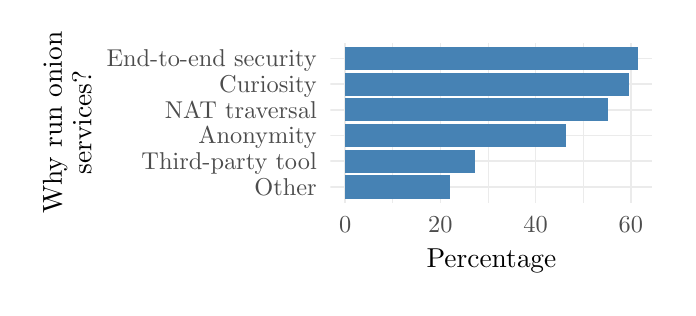
\begin{tikzpicture}[x=1pt,y=1pt]
\definecolor{fillColor}{RGB}{255,255,255}
\path[use as bounding box,fill=fillColor,fill opacity=0.00] (0,0) rectangle (231.26, 93.95);
\begin{scope}
\path[clip] (109.42, 30.77) rectangle (225.76, 88.45);
\definecolor{drawColor}{gray}{0.92}

\path[draw=drawColor,line width= 0.3pt,line join=round] (131.91, 30.77) --
	(131.91, 88.45);

\path[draw=drawColor,line width= 0.3pt,line join=round] (166.33, 30.77) --
	(166.33, 88.45);

\path[draw=drawColor,line width= 0.3pt,line join=round] (200.75, 30.77) --
	(200.75, 88.45);

\path[draw=drawColor,line width= 0.6pt,line join=round] (109.42, 36.35) --
	(225.76, 36.35);

\path[draw=drawColor,line width= 0.6pt,line join=round] (109.42, 45.66) --
	(225.76, 45.66);

\path[draw=drawColor,line width= 0.6pt,line join=round] (109.42, 54.96) --
	(225.76, 54.96);

\path[draw=drawColor,line width= 0.6pt,line join=round] (109.42, 64.26) --
	(225.76, 64.26);

\path[draw=drawColor,line width= 0.6pt,line join=round] (109.42, 73.57) --
	(225.76, 73.57);

\path[draw=drawColor,line width= 0.6pt,line join=round] (109.42, 82.87) --
	(225.76, 82.87);

\path[draw=drawColor,line width= 0.6pt,line join=round] (114.70, 30.77) --
	(114.70, 88.45);

\path[draw=drawColor,line width= 0.6pt,line join=round] (149.12, 30.77) --
	(149.12, 88.45);

\path[draw=drawColor,line width= 0.6pt,line join=round] (183.54, 30.77) --
	(183.54, 88.45);

\path[draw=drawColor,line width= 0.6pt,line join=round] (217.96, 30.77) --
	(217.96, 88.45);
\definecolor{fillColor}{RGB}{70,130,180}

\path[fill=fillColor] (114.70, 32.17) rectangle (152.48, 40.54);

\path[fill=fillColor] (114.70, 41.47) rectangle (161.72, 49.84);

\path[fill=fillColor] (114.70, 50.77) rectangle (194.45, 59.15);

\path[fill=fillColor] (114.70, 60.08) rectangle (209.56, 68.45);

\path[fill=fillColor] (114.70, 69.38) rectangle (217.12, 77.75);

\path[fill=fillColor] (114.70, 78.68) rectangle (220.48, 87.06);
\end{scope}
\begin{scope}
\path[clip] (  0.00,  0.00) rectangle (231.26, 93.95);
\definecolor{drawColor}{gray}{0.30}

\node[text=drawColor,anchor=base east,inner sep=0pt, outer sep=0pt, scale=  0.88] at (104.47, 33.32) {Other};

\node[text=drawColor,anchor=base east,inner sep=0pt, outer sep=0pt, scale=  0.88] at (104.47, 42.63) {Third-party tool};

\node[text=drawColor,anchor=base east,inner sep=0pt, outer sep=0pt, scale=  0.88] at (104.47, 51.93) {Anonymity};

\node[text=drawColor,anchor=base east,inner sep=0pt, outer sep=0pt, scale=  0.88] at (104.47, 61.23) {NAT traversal};

\node[text=drawColor,anchor=base east,inner sep=0pt, outer sep=0pt, scale=  0.88] at (104.47, 70.54) {Curiosity};

\node[text=drawColor,anchor=base east,inner sep=0pt, outer sep=0pt, scale=  0.88] at (104.47, 79.84) {End-to-end security};
\end{scope}
\begin{scope}
\path[clip] (  0.00,  0.00) rectangle (231.26, 93.95);
\definecolor{drawColor}{gray}{0.30}

\node[text=drawColor,anchor=base,inner sep=0pt, outer sep=0pt, scale=  0.88] at (114.70, 19.76) {0};

\node[text=drawColor,anchor=base,inner sep=0pt, outer sep=0pt, scale=  0.88] at (149.12, 19.76) {20};

\node[text=drawColor,anchor=base,inner sep=0pt, outer sep=0pt, scale=  0.88] at (183.54, 19.76) {40};

\node[text=drawColor,anchor=base,inner sep=0pt, outer sep=0pt, scale=  0.88] at (217.96, 19.76) {60};
\end{scope}
\begin{scope}
\path[clip] (  0.00,  0.00) rectangle (231.26, 93.95);
\definecolor{drawColor}{RGB}{0,0,0}

\node[text=drawColor,anchor=base,inner sep=0pt, outer sep=0pt, scale=  0.99] at (167.59,  7.44) {Percentage};
\end{scope}
\begin{scope}
\path[clip] (  0.00,  0.00) rectangle (231.26, 93.95);
\definecolor{drawColor}{RGB}{0,0,0}

\node[text=drawColor,rotate= 90.00,anchor=base,inner sep=0pt, outer sep=0pt, scale=  0.99] at ( 12.32, 59.61) {Why run onion};

\node[text=drawColor,rotate= 90.00,anchor=base,inner sep=0pt, outer sep=0pt, scale=  0.99] at ( 23.01, 59.61) {services?};
\end{scope}
\end{tikzpicture}

    \caption{The (multiple-choice) reasons our respondents have for running
    onion services.}
    \label{fig:onion-operation-reasons}
\end{figure}

\Cref{fig:onion-operation-concerns} illustrates the concerns that onion service
operators experience.  We consider three attacks; \first~somebody setting up a
phishing site for the operator's site, \second~a denial-of-service attack, and
\third~a deanonymization attack.  More than half of our respondents are at least
somewhat concerned about all of these attacks.  Almost 40\% claim to be
extremely concerned about somebody deanonymizing their onion service.  Indeed,
many respondents lamented the difficulty of protecting onion services from
application-layer deanonymization attacks.  Matic \ea\ demonstrated some of
these issues in 2015~\cite{Matic2015a}.

\begin{figure}[t]
    \centering
    % Created by tikzDevice version 0.10.1 on 2018-02-09 14:59:34
% !TEX encoding = UTF-8 Unicode
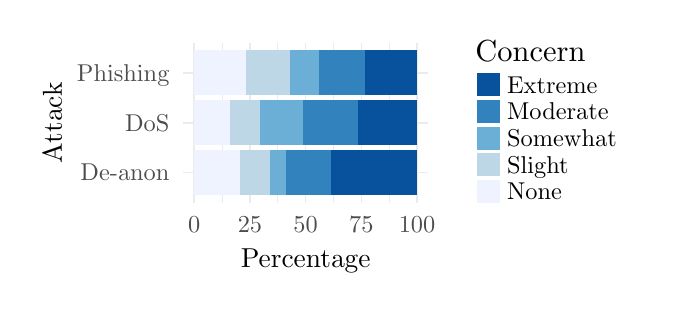
\begin{tikzpicture}[x=1pt,y=1pt]
\definecolor{fillColor}{RGB}{255,255,255}
\path[use as bounding box,fill=fillColor,fill opacity=0.00] (0,0) rectangle (224.04, 93.95);
\begin{scope}
\path[clip] ( 56.18, 30.77) rectangle (144.74, 88.45);
\definecolor{drawColor}{gray}{0.92}

\path[draw=drawColor,line width= 0.3pt,line join=round] ( 70.26, 30.77) --
	( 70.26, 88.45);

\path[draw=drawColor,line width= 0.3pt,line join=round] ( 90.39, 30.77) --
	( 90.39, 88.45);

\path[draw=drawColor,line width= 0.3pt,line join=round] (110.52, 30.77) --
	(110.52, 88.45);

\path[draw=drawColor,line width= 0.3pt,line join=round] (130.64, 30.77) --
	(130.64, 88.45);

\path[draw=drawColor,line width= 0.6pt,line join=round] ( 56.18, 41.59) --
	(144.74, 41.59);

\path[draw=drawColor,line width= 0.6pt,line join=round] ( 56.18, 59.61) --
	(144.74, 59.61);

\path[draw=drawColor,line width= 0.6pt,line join=round] ( 56.18, 77.64) --
	(144.74, 77.64);

\path[draw=drawColor,line width= 0.6pt,line join=round] ( 60.20, 30.77) --
	( 60.20, 88.45);

\path[draw=drawColor,line width= 0.6pt,line join=round] ( 80.33, 30.77) --
	( 80.33, 88.45);

\path[draw=drawColor,line width= 0.6pt,line join=round] (100.45, 30.77) --
	(100.45, 88.45);

\path[draw=drawColor,line width= 0.6pt,line join=round] (120.58, 30.77) --
	(120.58, 88.45);

\path[draw=drawColor,line width= 0.6pt,line join=round] (140.71, 30.77) --
	(140.71, 88.45);
\definecolor{fillColor}{RGB}{239,243,255}

\path[fill=fillColor] ( 60.20, 33.48) rectangle ( 76.78, 49.70);
\definecolor{fillColor}{RGB}{189,215,231}

\path[fill=fillColor] ( 76.78, 33.48) rectangle ( 87.44, 49.70);
\definecolor{fillColor}{RGB}{107,174,214}

\path[fill=fillColor] ( 87.44, 33.48) rectangle ( 93.35, 49.70);
\definecolor{fillColor}{RGB}{49,130,189}

\path[fill=fillColor] ( 93.35, 33.48) rectangle (109.54, 49.70);
\definecolor{fillColor}{RGB}{8,81,156}

\path[fill=fillColor] (109.54, 33.48) rectangle (140.72, 49.70);
\definecolor{fillColor}{RGB}{239,243,255}

\path[fill=fillColor] ( 60.20, 51.50) rectangle ( 73.16, 67.72);
\definecolor{fillColor}{RGB}{189,215,231}

\path[fill=fillColor] ( 73.16, 51.50) rectangle ( 83.77, 67.72);
\definecolor{fillColor}{RGB}{107,174,214}

\path[fill=fillColor] ( 83.77, 51.50) rectangle ( 99.47, 67.72);
\definecolor{fillColor}{RGB}{49,130,189}

\path[fill=fillColor] ( 99.47, 51.50) rectangle (119.50, 67.72);
\definecolor{fillColor}{RGB}{8,81,156}

\path[fill=fillColor] (119.50, 51.50) rectangle (140.71, 67.72);
\definecolor{fillColor}{RGB}{239,243,255}

\path[fill=fillColor] ( 60.20, 69.53) rectangle ( 79.05, 85.75);
\definecolor{fillColor}{RGB}{189,215,231}

\path[fill=fillColor] ( 79.05, 69.53) rectangle ( 94.75, 85.75);
\definecolor{fillColor}{RGB}{107,174,214}

\path[fill=fillColor] ( 94.75, 69.53) rectangle (105.36, 85.75);
\definecolor{fillColor}{RGB}{49,130,189}

\path[fill=fillColor] (105.36, 69.53) rectangle (121.85, 85.75);
\definecolor{fillColor}{RGB}{8,81,156}

\path[fill=fillColor] (121.85, 69.53) rectangle (140.70, 85.75);
\end{scope}
\begin{scope}
\path[clip] (  0.00,  0.00) rectangle (224.04, 93.95);
\definecolor{drawColor}{gray}{0.30}

\node[text=drawColor,anchor=base east,inner sep=0pt, outer sep=0pt, scale=  0.88] at ( 51.23, 38.56) {De-anon};

\node[text=drawColor,anchor=base east,inner sep=0pt, outer sep=0pt, scale=  0.88] at ( 51.23, 56.58) {DoS};

\node[text=drawColor,anchor=base east,inner sep=0pt, outer sep=0pt, scale=  0.88] at ( 51.23, 74.61) {Phishing};
\end{scope}
\begin{scope}
\path[clip] (  0.00,  0.00) rectangle (224.04, 93.95);
\definecolor{drawColor}{gray}{0.30}

\node[text=drawColor,anchor=base,inner sep=0pt, outer sep=0pt, scale=  0.88] at ( 60.20, 19.76) {0};

\node[text=drawColor,anchor=base,inner sep=0pt, outer sep=0pt, scale=  0.88] at ( 80.33, 19.76) {25};

\node[text=drawColor,anchor=base,inner sep=0pt, outer sep=0pt, scale=  0.88] at (100.45, 19.76) {50};

\node[text=drawColor,anchor=base,inner sep=0pt, outer sep=0pt, scale=  0.88] at (120.58, 19.76) {75};

\node[text=drawColor,anchor=base,inner sep=0pt, outer sep=0pt, scale=  0.88] at (140.71, 19.76) {100};
\end{scope}
\begin{scope}
\path[clip] (  0.00,  0.00) rectangle (224.04, 93.95);
\definecolor{drawColor}{RGB}{0,0,0}

\node[text=drawColor,anchor=base,inner sep=0pt, outer sep=0pt, scale=  0.99] at (100.46,  7.44) {Percentage};
\end{scope}
\begin{scope}
\path[clip] (  0.00,  0.00) rectangle (224.04, 93.95);
\definecolor{drawColor}{RGB}{0,0,0}

\node[text=drawColor,rotate= 90.00,anchor=base,inner sep=0pt, outer sep=0pt, scale=  0.99] at ( 12.32, 59.61) {Attack};
\end{scope}
\begin{scope}
\path[clip] (  0.00,  0.00) rectangle (224.04, 93.95);
\definecolor{drawColor}{RGB}{0,0,0}

\node[text=drawColor,anchor=base west,inner sep=0pt, outer sep=0pt, scale=  1.10] at (161.81, 81.72) {Concern};
\end{scope}
\begin{scope}
\path[clip] (  0.00,  0.00) rectangle (224.04, 93.95);
\definecolor{fillColor}{RGB}{8,81,156}

\path[fill=fillColor] (162.52, 69.18) rectangle (170.74, 77.40);
\end{scope}
\begin{scope}
\path[clip] (  0.00,  0.00) rectangle (224.04, 93.95);
\definecolor{fillColor}{RGB}{49,130,189}

\path[fill=fillColor] (162.52, 59.55) rectangle (170.74, 67.76);
\end{scope}
\begin{scope}
\path[clip] (  0.00,  0.00) rectangle (224.04, 93.95);
\definecolor{fillColor}{RGB}{107,174,214}

\path[fill=fillColor] (162.52, 49.91) rectangle (170.74, 58.12);
\end{scope}
\begin{scope}
\path[clip] (  0.00,  0.00) rectangle (224.04, 93.95);
\definecolor{fillColor}{RGB}{189,215,231}

\path[fill=fillColor] (162.52, 40.27) rectangle (170.74, 48.49);
\end{scope}
\begin{scope}
\path[clip] (  0.00,  0.00) rectangle (224.04, 93.95);
\definecolor{fillColor}{RGB}{239,243,255}

\path[fill=fillColor] (162.52, 30.64) rectangle (170.74, 38.85);
\end{scope}
\begin{scope}
\path[clip] (  0.00,  0.00) rectangle (224.04, 93.95);
\definecolor{drawColor}{RGB}{0,0,0}

\node[text=drawColor,anchor=base west,inner sep=0pt, outer sep=0pt, scale=  0.88] at (173.26, 70.26) {Extreme};
\end{scope}
\begin{scope}
\path[clip] (  0.00,  0.00) rectangle (224.04, 93.95);
\definecolor{drawColor}{RGB}{0,0,0}

\node[text=drawColor,anchor=base west,inner sep=0pt, outer sep=0pt, scale=  0.88] at (173.26, 60.62) {Moderate};
\end{scope}
\begin{scope}
\path[clip] (  0.00,  0.00) rectangle (224.04, 93.95);
\definecolor{drawColor}{RGB}{0,0,0}

\node[text=drawColor,anchor=base west,inner sep=0pt, outer sep=0pt, scale=  0.88] at (173.26, 50.99) {Somewhat};
\end{scope}
\begin{scope}
\path[clip] (  0.00,  0.00) rectangle (224.04, 93.95);
\definecolor{drawColor}{RGB}{0,0,0}

\node[text=drawColor,anchor=base west,inner sep=0pt, outer sep=0pt, scale=  0.88] at (173.26, 41.35) {Slight};
\end{scope}
\begin{scope}
\path[clip] (  0.00,  0.00) rectangle (224.04, 93.95);
\definecolor{drawColor}{RGB}{0,0,0}

\node[text=drawColor,anchor=base west,inner sep=0pt, outer sep=0pt, scale=  0.88] at (173.26, 31.71) {None};
\end{scope}
\end{tikzpicture}

    \caption{The level of concern onion service operators have with respect to a
    phishing clone of their service, denial-of-service attacks, and
    deanonymization.}
    \label{fig:onion-operation-concerns}
\end{figure}

\subsubsection{Vanity domains are a double-edged sword}

Phishing remains an issue despite onion services' extra anonymity and security
properties.  Past work has documented phishing onion sites that transparently
rewrote Bitcoin addresses to hijack Bitcoin
transactions~\cite{Winter2016a,Nurmi2015a,Monteiro2016a}.  Key to this attack is
the difficulty of telling apart an authentic onion domain from an impersonation.
For conventional domains we rely on (\textsc{ev}) certificates, browser
protections, search results, and long-lived reputation, but none of these
methods have matured for onion services.  Does the nature of onion services
facilitate phishing attacks?  If so, what can we do to mitigate the issue?

We asked our respondents if they ever thought about the authenticity of an onion
site.  The majority of our respondents (80\%) did while 20\% did not.  Clearly,
there is a need for verification, but how does one verify that an onion service
is authentic?  \Cref{fig:determining-legitimacy} gives an overview of the
strategies that our respondents employ.  More than half either consult trusted
sources (\eg, friends or another, trusted web site) or use bookmarks when
revisiting onion services.  Many respondents also verify the domain in the
browser's address bar (46\%), check if the corresponding web site has a link to
its onion site (41\%), or hope that the onion service has an \textsc{https}
certificate (36\%).\footnote{DigiCert is issuing \textsc{ev} certificates for
onion sites~\cite{DigiCert2015a}, but adoption has been slow---presumably in part
because \textsc{ev} certificates require the \textsc{ca} to verify the
applicant's identity and they are not free.}  Alarmingly, almost 30\% of
respondents stated that they sometimes cannot tell the difference between an
authentic service and an impersonation, and 11\% never check a service's
legitimacy in the first place.  People who selected ``Other'' provided a wide
variety of ad-hoc phishing protections, some of which are clearly misguided,
further highlighting the importance of this issue.

\begin{figure}[t]
    \centering
    % Created by tikzDevice version 0.10.1 on 2018-01-12 16:30:02
% !TEX encoding = UTF-8 Unicode
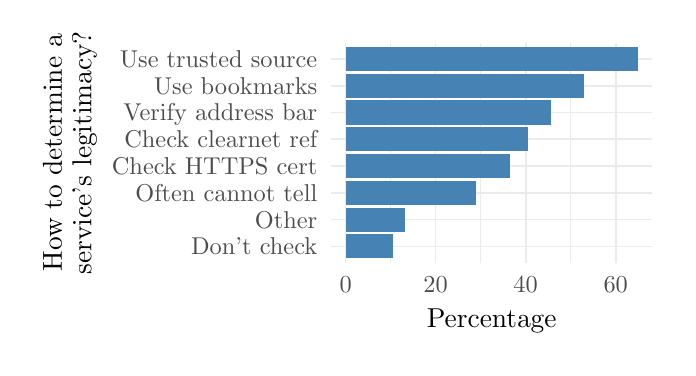
\begin{tikzpicture}[x=1pt,y=1pt]
\definecolor{fillColor}{RGB}{255,255,255}
\path[use as bounding box,fill=fillColor,fill opacity=0.00] (0,0) rectangle (231.26,115.63);
\begin{scope}
\path[clip] (109.60, 30.77) rectangle (225.76,110.13);
\definecolor{drawColor}{gray}{0.92}

\path[draw=drawColor,line width= 0.3pt,line join=round] (131.15, 30.77) --
	(131.15,110.13);

\path[draw=drawColor,line width= 0.3pt,line join=round] (163.68, 30.77) --
	(163.68,110.13);

\path[draw=drawColor,line width= 0.3pt,line join=round] (196.21, 30.77) --
	(196.21,110.13);

\path[draw=drawColor,line width= 0.6pt,line join=round] (109.60, 36.58) --
	(225.76, 36.58);

\path[draw=drawColor,line width= 0.6pt,line join=round] (109.60, 46.26) --
	(225.76, 46.26);

\path[draw=drawColor,line width= 0.6pt,line join=round] (109.60, 55.94) --
	(225.76, 55.94);

\path[draw=drawColor,line width= 0.6pt,line join=round] (109.60, 65.61) --
	(225.76, 65.61);

\path[draw=drawColor,line width= 0.6pt,line join=round] (109.60, 75.29) --
	(225.76, 75.29);

\path[draw=drawColor,line width= 0.6pt,line join=round] (109.60, 84.97) --
	(225.76, 84.97);

\path[draw=drawColor,line width= 0.6pt,line join=round] (109.60, 94.65) --
	(225.76, 94.65);

\path[draw=drawColor,line width= 0.6pt,line join=round] (109.60,104.33) --
	(225.76,104.33);

\path[draw=drawColor,line width= 0.6pt,line join=round] (114.88, 30.77) --
	(114.88,110.13);

\path[draw=drawColor,line width= 0.6pt,line join=round] (147.41, 30.77) --
	(147.41,110.13);

\path[draw=drawColor,line width= 0.6pt,line join=round] (179.95, 30.77) --
	(179.95,110.13);

\path[draw=drawColor,line width= 0.6pt,line join=round] (212.48, 30.77) --
	(212.48,110.13);
\definecolor{fillColor}{RGB}{70,130,180}

\path[fill=fillColor] (114.88, 32.22) rectangle (131.91, 40.93);

\path[fill=fillColor] (114.88, 41.90) rectangle (136.32, 50.61);

\path[fill=fillColor] (114.88, 51.58) rectangle (162.17, 60.29);

\path[fill=fillColor] (114.88, 61.26) rectangle (174.14, 69.97);

\path[fill=fillColor] (114.88, 70.94) rectangle (180.76, 79.65);

\path[fill=fillColor] (114.88, 80.61) rectangle (188.96, 89.32);

\path[fill=fillColor] (114.88, 90.29) rectangle (200.95, 99.00);

\path[fill=fillColor] (114.88, 99.97) rectangle (220.48,108.68);
\end{scope}
\begin{scope}
\path[clip] (  0.00,  0.00) rectangle (231.26,115.63);
\definecolor{drawColor}{gray}{0.30}

\node[text=drawColor,anchor=base east,inner sep=0pt, outer sep=0pt, scale=  0.88] at (104.65, 33.55) {Don't check};

\node[text=drawColor,anchor=base east,inner sep=0pt, outer sep=0pt, scale=  0.88] at (104.65, 43.23) {Other};

\node[text=drawColor,anchor=base east,inner sep=0pt, outer sep=0pt, scale=  0.88] at (104.65, 52.91) {Often cannot tell};

\node[text=drawColor,anchor=base east,inner sep=0pt, outer sep=0pt, scale=  0.88] at (104.65, 62.58) {Check HTTPS cert};

\node[text=drawColor,anchor=base east,inner sep=0pt, outer sep=0pt, scale=  0.88] at (104.65, 72.26) {Check clearnet ref};

\node[text=drawColor,anchor=base east,inner sep=0pt, outer sep=0pt, scale=  0.88] at (104.65, 81.94) {Verify address bar};

\node[text=drawColor,anchor=base east,inner sep=0pt, outer sep=0pt, scale=  0.88] at (104.65, 91.62) {Use bookmarks};

\node[text=drawColor,anchor=base east,inner sep=0pt, outer sep=0pt, scale=  0.88] at (104.65,101.29) {Use trusted source};
\end{scope}
\begin{scope}
\path[clip] (  0.00,  0.00) rectangle (231.26,115.63);
\definecolor{drawColor}{gray}{0.30}

\node[text=drawColor,anchor=base,inner sep=0pt, outer sep=0pt, scale=  0.88] at (114.88, 19.76) {0};

\node[text=drawColor,anchor=base,inner sep=0pt, outer sep=0pt, scale=  0.88] at (147.41, 19.76) {20};

\node[text=drawColor,anchor=base,inner sep=0pt, outer sep=0pt, scale=  0.88] at (179.95, 19.76) {40};

\node[text=drawColor,anchor=base,inner sep=0pt, outer sep=0pt, scale=  0.88] at (212.48, 19.76) {60};
\end{scope}
\begin{scope}
\path[clip] (  0.00,  0.00) rectangle (231.26,115.63);
\definecolor{drawColor}{RGB}{0,0,0}

\node[text=drawColor,anchor=base,inner sep=0pt, outer sep=0pt, scale=  0.99] at (167.68,  7.44) {Percentage};
\end{scope}
\begin{scope}
\path[clip] (  0.00,  0.00) rectangle (231.26,115.63);
\definecolor{drawColor}{RGB}{0,0,0}

\node[text=drawColor,rotate= 90.00,anchor=base,inner sep=0pt, outer sep=0pt, scale=  0.99] at ( 12.32, 70.45) {How to determine a};

\node[text=drawColor,rotate= 90.00,anchor=base,inner sep=0pt, outer sep=0pt, scale=  0.99] at ( 23.01, 70.45) {service's legitimacy?};
\end{scope}
\end{tikzpicture}

    \caption{How our respondents determine an onion service's legitimacy.}
    \label{fig:determining-legitimacy}
\end{figure}

Originally meant to provide ``branding'' for an onion service, vanity onion
domains also play a role in the context of phishing.  There is concern that the
short and recognizable prefixes tempt users to only verify the prefix and ignore
subsequent characters~\cite{Winter2015a}.  Quoting two of our survey responses:

\begin{displayquote}[Survey respondent]
I only memorize the first part of the domain.
\end{displayquote}

\begin{displayquote}[Survey respondent]
If there isn't some cognizable word at the start, it'll be more difficult for me
to determine if I'm going to the correct domain or a scam. I may end up going to
less .onion sites as a result.
\end{displayquote}

Focusing only on the vanity part of a domain allows attackers to create an
impersonation domain that features the original's prefix but differs in
subsequent characters.  Nurmi~\cite{Nurmi2015a} and
Monteiro~\cite{Monteiro2016a} have both documented such an attack, but its
effectiveness is not known.

The majority of our respondents appreciate vanity domains because they are easy
to remember (64\%) and easy to recognize (64\%), and they provide a unique
``branding'' (34\%).  Some respondents indicate that a vanity prefix---like a
traditional domain---informs about an onion service's content, letting visitors
know what to expect and thus preventing unpleasant surprises.  Only 8\% dislike vanity
onion domains, and 15\% do not have an opinion.  Interestingly, some respondents
consider vanity domains economically unfair because wealthy entities can afford
to generate longer prefixes.  Several respondents also voiced their concern that
vanity domains create a false sense of security and facilitate phishing attacks.

In a separate question, we inquired how many characters our respondents verify in
onion domains.  43\% verify thirteen to sixteen digits, \ie, (almost) the full
domain, while 46\% verify up to nine digits, which is within the realm of brute
force attacks.  Finally, a handful of respondents cited misguided reasons why
they dislike vanity domains, \eg, some believe that vanity domains are a sign of
weak hash functions while others believe that vanity domains make the onion
service ``less hidden'' or allow somebody to create ``the same private key.''
